\documentclass[11pt]{article}
\usepackage[sort]{natbib}
\usepackage{bm,amsmath,bbm,amsfonts,nicefrac,latexsym,amsmath,amsfonts,amsbsy,amscd,amsxtra,amsgen,amsopn,bbm,amsthm,amssymb,graphicx, color, caption, subcaption}
\usepackage{fancyhdr, pbox}
\usepackage[margin=0.8in]{geometry}
\usepackage[english]{babel}
\usepackage[section]{placeins}
\usepackage{wrapfig}
\usepackage{lscape}
\usepackage{rotating}
\usepackage{epstopdf}
\bibliographystyle{plainnat}

\title{Investigating the role of \textbf{R} and \textbf{B} in improving a model of forest carbon balance using 4D-Var.}
\author{Ewan Pinnington}

\newtheorem{theorem}{Theorem}[section]
\newtheorem*{defn}{Definition}


\begin{document}

\maketitle

\section*{Abstract}

Efforts to implement functional ecology and land surface models in variational data assimilation routines have been limited with sequential and Markov chain Monte Carlo data assimilation methods being more prevalent. When data assimilation has been used with models of carbon balance, background errors (describing our knowledge of error in our prior model estimates before data assimilation) and observation errors have largely been treated as independent and uncorrelated. In numerical weather prediction it has been shown that including correlations in these errors can considerably improve data assimilation results and forecasts. In this paper we implement a simple model of forest carbon balance in a Four-Dimensional Variational (4D-Var) data assimilation scheme, for parameter and state estimation, assimilating observations of Net Ecosystem Exchange (NEE) taken at the Alice Holt flux site in Hampshire managed by Forest Research. We then investigate the effect of specifying correlations between parameter and state variables in background errors and the effect of specifying correlations in time between observation errors. We do this by moving away from a diagonal representation of the background error covariance matrix, \textbf{B}, and the observation error covariance matrix, \textbf{R}. We outline novel methods for creating a correlated \textbf{B} and \textbf{R} and show that using these new correlated matrices can almost half the root mean square error in our models forecast of NEE in comparison to the results when using an uncorrelated diagonal \textbf{B} and \textbf{R}.      

\section{Introdution}

\subsection{Tree blurb}
Terrestrial ecosystems and oceans are responsible for removing around half of all human emitted carbon-dioxide from the atmosphere and therefore greatly reduce the effect of anthropogenic induced climate change. Terrestrial ecosystem carbon uptake is the least understood process in the global carbon cycle \citep{ciais2014carbon}. It is therefore vital that we improve understanding of the carbon uptake of terrestrial ecosystems and their response to climate change in order to better constrain predictions of future carbon budgets. Observations of the Net Ecosystem Exchange (NEE) of CO$_{2}$ between terestrial ecosystems and the atmosphere are now routinely made at flux tower sites world-wide \citep{baldocchi2008turner} providing a great resource for model validation and data assimilation.

\subsection{DA paragraph}
Data assimilation is the process of combining a mathematical model with observations in order to improve the estimate of the state of a system. Data assimilation has been used in many applications with great results for improving models and forecast. One such application has been In numerical weather prediction where the impact of data assimilation has been vast with the four day forecast in 2014 having the same level of accuracy as the one day forecast when data assimilation was first introduced operationally in 1979 \citep{rabier2005overview, kalnay2003atmospheric}. This increase in forecast skill is obviously not solely due to data assimilation but also increased quality and resolution of observations along with improvements in model structure. However the introduction and evolution of data assimilation has played a large part. The current method implemented at several leading operational numerical weather prediction centres is Four-Dimensional Variational data assimilation (4D-Var), which has been shown to be a significant improvement over its predecessor three-dimensional variational assimilation \citep{lorenc2005does}. Variational assimilation techniques minimise a cost function to find an improved state of a system. The minimisation routine requires the derivative of the model, this can sometimes prove a problem to find. However using techniques such as automatic-differentiation can reduce the time taken to implement the derivative of a model and also increase the accuracy of the models derivative.

\subsection{DALEC and ecosystem models with data assimilation (draw out gaps):}
Many different observations relevant to the carbon balance of forests have now been combined with functional ecology models, using data assimilation, in order to improve our knowledge ecological systems \citep{zobitz2011primer, fox2009reflex}. Two such models that have been used extensively with data assimilation are the Data Assimilation Linked Ecosystem Carbon (DALEC) model \citep{williams2005improved} and the Simplified Photosynthesis and Evapo-Transpiration (SIPNET) model \citep{braswell2005estimating}, nearly all data assimilation routines built with these models have used sequential and Monte Carlo Markov chain (MCMC) data assimilation methods with the exception of DALEC being implemented in a variational routine by \citet{delahaies2013regularization}. There have been examples of global land surface models being implemented with variational methods such as the Carbon Cycle Data Assimilation System (CCDAS) \citep{Kaminski2013} and the global model ORganizing Carbon and Hydrology In Dynamic EcosystEms (ORCHIDEE) \citep{Krinner2005}. These examples have mainly been used to assimilate data from satellite observations with a few examples where site level data has been assimilated \citep{Verbeeck2011, Bacour2015}.

Currently background and observation errors have been treated as uncorrelated and independent in ecosystem model data assimilation schemes. In many data assimilation schemes background and observation errors are represented by the error covariance matrices \textbf{B} and \textbf{R} respectively. The off-diagonal elements of these matrices indicate the correlations between the parameter and state variables for \textbf{B} and the correlations between observation errors for \textbf{R}. Including correlations in both \textbf{B} and \textbf{R} has been shown to significantly improve data assimilation results in numerical weather prediction, with much more research ongoing in this field \citep{fisher2003background, Stewart2013}. Although correlations in \textbf{R} have been explored in numerical weather prediction, currently these have been mainly between observations made at the the same time rather than correlations between observations throughout time. In \citet{richardson2010estimating} the problem of data streams with many more observations having more impact on assimilation results than those with fewer observations is discussed and an assimilation method put forward to deal with this. Specifying serial correlations between observations of the same quantity decreases the impact of these observations \citep{jarvinen1999variational} and represents another way to tackle this problem, whilst also adding valuable information to our data assimilation routine. 

\subsection{What does this paper do/results:}
In this paper we implement the new version of DALEC (DALEC2 \citep{Bloom2015}) in a 4DVAR data assimilation scheme for state and parameter estimation, assimilating daily NEE observations from the Alice Holt flux site in Hampshire managed by Forest Research. This assimilation scheme is then subjected to rigorous testing to ensure correctness. We then outline a new method for including parameter and state correlations in our background error covariance matrix and a method for including serial correlations in our observation error covariance matrix. These matrices are then used in a series of experiments in order to examine the effect that including correlations in our assimilation scheme has on our results. We show that specifying parameter and state correlations in our prior knowledge and serial correlations between observation errors can drastically improve the results from our assimilation.

\section{Model and Data Assimilation Methods}

\subsection{Alice Holt research forest}

Alice Holt is a well established research forest located in Hampshire, England with observational data spanning 50 years, the site is managed by Forest Research. The flux tower site is situated in the Straits Inclosure which is a mainly deciduous part of the forest comprising of mostly oak trees with a hazel understory, although there is a bank of conifer approximately 1km north west of the flux tower site. Flux tower records of Net Ecosystem Exchange (NEE) are available from 1999 up to present day, meaning that Alice Holt has one of the longest records of flux tower data in the UK.  

\subsection{The DALEC2 model}

The DALEC2 model is a simple process-based model describing the carbon balance of a forest ecosystem \citep{Bloom2015} and is the new version of the original DALEC \citep{williams2005improved}. The model is constructed of six carbon pools (labile ($C_{lab}$), foliage ($C_f$), fine roots ($C_r$), woody stems and coarse roots ($C_w$), fresh leaf and fine root litter ($C_l$) and soil organic matter and coarse woody debris ($C_s$)) linked via fluxes. The aggregated canopy model (ACM) \citep{williams1997predicting} is used to calculate daily gross primary production ($GPP$) of the forest, taking meteorological driving data and the site's leaf area index (a function of $C_f$) as arguments.   

\begin{figure}[ht]
    \centering
    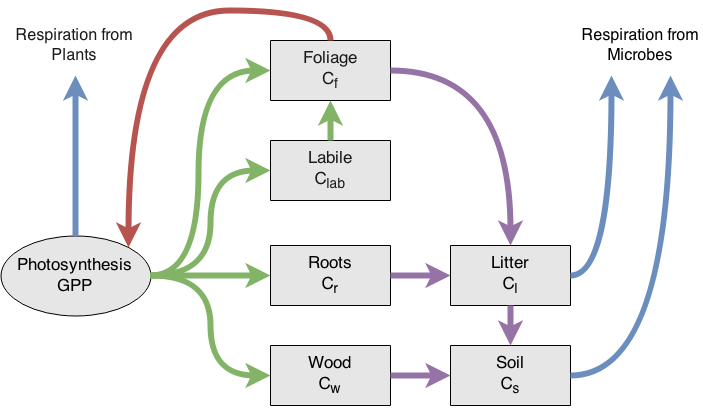
\includegraphics[width=0.5\textwidth]{Dalecdiagram.png}
    \caption{Representation of the fluxes in the DALEC2 carbon balance model. Green arrows represent C allocation, purple arrows represent litter fall and decomposition fluxes, blue arrows represent respiration fluxes and the red arrow represents the feedback of foliar carbon to the $GPP$ function.}
    \label{fig:DALEC_mod}
\end{figure}

The model equations for the carbon pools at day $t+1$ are as follows:

\begin{align}
GPP^{t} &= ACM(C_f^{t}, c_{lma}, c_{eff}, \Psi) \label{GPP}
\\C_{lab}^{t+1}&=(1-\Phi _{on})C_{lab}^{t}+(1-f_{auto})(1-f_{fol})f_{lab}GPP^{t}, \label{daleclab}
\\C_f^{t+1}&=(1-\Phi_{off})C_f^{t}+\Phi_{on}C_{lab}^{t}+(1-f_{auto})f_{fol}GPP^{t}, \label{dalec1}
\\C_r^{t+1}&=(1-\theta_{roo})C_r^{t}+(1-f_{auto})(1-f_{fol})(1-f_{lab})f_{roo}GPP^{t}, 
\\C_w^{t+1}&=(1-\theta_{woo})C_w^{t}+(1-f_{auto})(1-f_{fol})(1-f_{lab})(1-f_{roo})GPP^{t}, 
\\C_l^{t+1}&=(1-(\theta_{lit}+\theta_{min})e^{\Theta T^{t}})C_l^{t}+\theta_{roo}C_r^{t}+\Phi_{off}C_f^{t}, 
\\C_s^{t+1}&=(1-\theta_{som}e^{\Theta T^{t}})C_s^{t}+\theta_{woo}C_w^{t}+\theta_{min}e^{\Theta T^{t}}C_l^{t}, \label{dalec5}
\end{align}

where $T^{t}$ is the daily mean temperature, $\Psi$ represents the meteorological driving data used in the $GPP$ function and $\Phi_{on} / \Phi_{off}$ are functions controlling leaf on and leaf off. The model parameters used in equations \ref{GPP} to \ref{dalec5} and the equations used to calculate $GPP$, $\Phi_{on}$ and $\Phi_{off}$ are included in the appendix. The full details of this version of DALEC can be found in \cite{Bloom2015}.

\subsection{4D-Var} \label{4dvar}

In 4D-Var we aim to maximise the probability of the initial state $\textbf{x}_0$ given a set of observations $\textbf{y}$, $P(\textbf{x}_0|\textbf{y})$, over some time window, $N$. $P(\textbf{x}_0|\textbf{y})$ is maximised by minimising a cost function $J(\textbf{x})$ derived from Bayes Theorem \citep{lewis2006dynamic}. The cost function is given as,

\begin{equation}
J(\textbf{x}_0) = \frac{1}{2}(\textbf{x}_0-\textbf{x}_b)^{T}\textbf{B}^{-1}(\textbf{x}_0-\textbf{x}_b)+\frac{1}{2}\sum_{i=0}^{N}(\textbf{y}_i-h_i(\textbf{x}_i))^{T}\textbf{R}_{i}^{-1}(\textbf{y}_i-h_i(\textbf{x}_i)),
\end{equation}

where $\textbf{x}_b$ is the background and acts as the initial guess to the state $\textbf{x}_0$, $\textbf{B}$ is the background error covariance matrix and quantifies our knowledge of the error in the background, $h_i$ is the observation operator at time $t_i$ and maps the state vector evolved by the nonlinear model ($m_{0\rightarrow i}(\mathbf{x}_{0})=\textbf{x}_i$) to the observations at this time ($\textbf{y}_i$) and $\textbf{R}_i$ is the observation error covariance matrix at time $t_i$ and represents our knowledge of the uncertainty in the observations. The state that minimises the cost function is called the analysis and is denoted as $\textbf{x}_a$, this state is found using a minimisation routine (here we use a truncated Newton method \citep{Nocedal1999} from the Python package Scipy.optimize) that takes the cost function, the initial guess ($\textbf{x}_b$) and also the gradient of the cost function given as,

\begin{equation}
\nabla J(\textbf{x}_0) = \textbf{B}^{-1}(\textbf{x}_0-\textbf{x}_b)-\sum_{i=0}^{N}\textbf{M}_{i,0}^{T}\textbf{H}_i^{T}\textbf{R}_{i}^{-1}(\textbf{y}_i-h_i(\textbf{x}_i)),
\end{equation}

where $\textbf{H}_i = \frac{\partial h_i(\textbf{x}_i)}{\partial\textbf{x}_i}$ is our linearized observation operator and $\mathbf{M}_{i,0}=\mathbf{M}_{i-1}\mathbf{M}_{i-2}\cdots\mathbf{M}_0$ is our tangent linear model with $\mathbf{M}_i=\frac{\partial m_{i}(\textbf{x}_{i})}{\partial \textbf{x}_{i}}$. We can rewrite the cost function and its gradient to avoid the sum notation as,

\begin{equation}
J(\textbf{x}_0) = \frac{1}{2}(\textbf{x}_0-\textbf{x}_b)^{T}\textbf{B}^{-1}(\textbf{x}_0-\textbf{x}_b)+\frac{1}{2}(\hat{\textbf{y}}-\hat{h}(\textbf{x}_0))^{T}\hat{\textbf{R}}^{-1}(\hat{\textbf{y}}-\hat{h}(\textbf{x}_0)) \label{costfn}
\end{equation}
and
\begin{equation}
\nabla J(\textbf{x}_0) = \textbf{B}^{-1}(\textbf{x}_0-\textbf{x}_b)-\hat{\mathbf{H}}^{T}\hat{\textbf{R}}^{-1}(\hat{\textbf{y}}-\hat{h}(\textbf{x}_0)), \label{gradcostfn}
\end{equation}
where,
\begin{equation}
\hat{\textbf{y}}=
\begin{pmatrix}
\textbf{y}_0 \\
\textbf{y}_1\\
\vdots \\
\textbf{y}_N
\end{pmatrix},
\hspace{1mm}
\hat{h}(\textbf{x}_0)=
\begin{pmatrix}
h_0(\textbf{x}_0) \\
h_1(m_{0\rightarrow 1}(\mathbf{x}_{0}))\\
\vdots \\
h_N(m_{0\rightarrow N}(\mathbf{x}_{0}))
\end{pmatrix},
\hspace{1mm}
\hat{\mathbf{R}}=
\begin{pmatrix}
\mathbf{R}_0 & 0 & 0 & 0 \\
0 & \mathbf{R}_1 & 0 & 0 \\
0 & 0 & \ddots & 0 \\
0 & 0 & 0 & \mathbf{R}_N
\end{pmatrix}
\hspace{1mm} \text{and} \hspace{3mm}
\hat{\mathbf{H}}=
\begin{pmatrix}
\mathbf{H}_0 \\
\mathbf{H}_1\mathbf{M}_0\\
\vdots \\
\mathbf{H}_N\mathbf{M}_{N,0}
\end{pmatrix}.
\end{equation}

Solving the cost function in this form will also allow us to build serial correlations into the observation error covariance matrix $\hat{\mathbf{R}}$.
%Forecast skill score, $SS = 1 - \frac{MSE_{forecast}}{MSE_{ref}}$, http://en.wikipedia.org/wiki/Forecast_skill

\subsection{Testing of 4D-Var system}

In our DALECV2 4D-Var scheme the state vector, $\textbf{x}_0$, corresponds to the vector of the 17 model parameters and 6 initial carbon pool values, which can be found in the appendix. In the following tests we use a diagonal approximation to our background and observational error covariance matrices so that, 
$\textbf{B}=\text{diag}(\underline{\sigma}_b^2)$ and $\hat{\textbf{R}}=\text{diag}(\underline{\sigma}_o^2 )$,
where $\underline{\sigma}_b$ and $\underline{\sigma}_o$ are the vectors of the background and observational standard deviations respectively.

In order to find the tangent linear model (TLM) for DALECV2 we need to find the derivative of the model at each time step with respect to the 17 model parameters and the 6 carbon pools. We use the AlgoPy automatic differentiation package in Python to calculate the TLM at each time step. This package uses forward mode automatic differentiation to calculate the derivative of our model. AlgoPy was selected after testing other automatic differentiation packages (PyAutoDiff and ad.py) and finding that AlgoPy could compute the TLM in the fastest time. We now have all the tools to create our 4D-Var scheme. In sections \ref{sec:testtlm} to \ref{sec:testgrad} we will show some tests of our scheme.

\subsubsection{Test of tangent linear model} \label{sec:testtlm}

We can have confidence that our implementation of the TLM for DALEC2 is correct as it passes relevant tests. In 4D-Var we assume the tangent linear hypothesis,
\begin{equation}
m_{0\rightarrow i}(\mathbf{x}_0+\gamma \delta\mathbf{x}_0) \approx m_{0 \rightarrow i}(\mathbf{x}_0) + \mathbf{M}_{i,0}\gamma \delta\mathbf{x}_0. \label{TLH}
\end{equation}
The validity of this assumption depends on how nonlinear the model is, the length of the assimilation window and the size of the perturbation $\delta\mathbf{x}_0$. We can test this by rearranging equation~\ref{TLH} to find the relative error,
\begin{equation}
E_R=\frac{||m_{0\rightarrow i}(\mathbf{x}_0+\gamma \delta\mathbf{x}_0) - m_{0 \rightarrow i}(\mathbf{x}_0)||}{||\mathbf{M}_{i,0}\gamma\delta\mathbf{x}_0||}, \label{tlmtest}
\end{equation}
where we should have $E_R \rightarrow 0$ as $\gamma \rightarrow 0$. In figure~\ref{fig:tlm} we have plotted equation~\ref{tlmtest} for DALEC2 with a TLM evolving our state 731 days forward in time for a $5\%$ perturbation $\delta \textbf{x}_0$. Figure~\ref{fig:tlm} shows that our TLM behaves as expected for values of $\gamma$ approaching $0$.


\begin{figure}[ht]
    \centering
    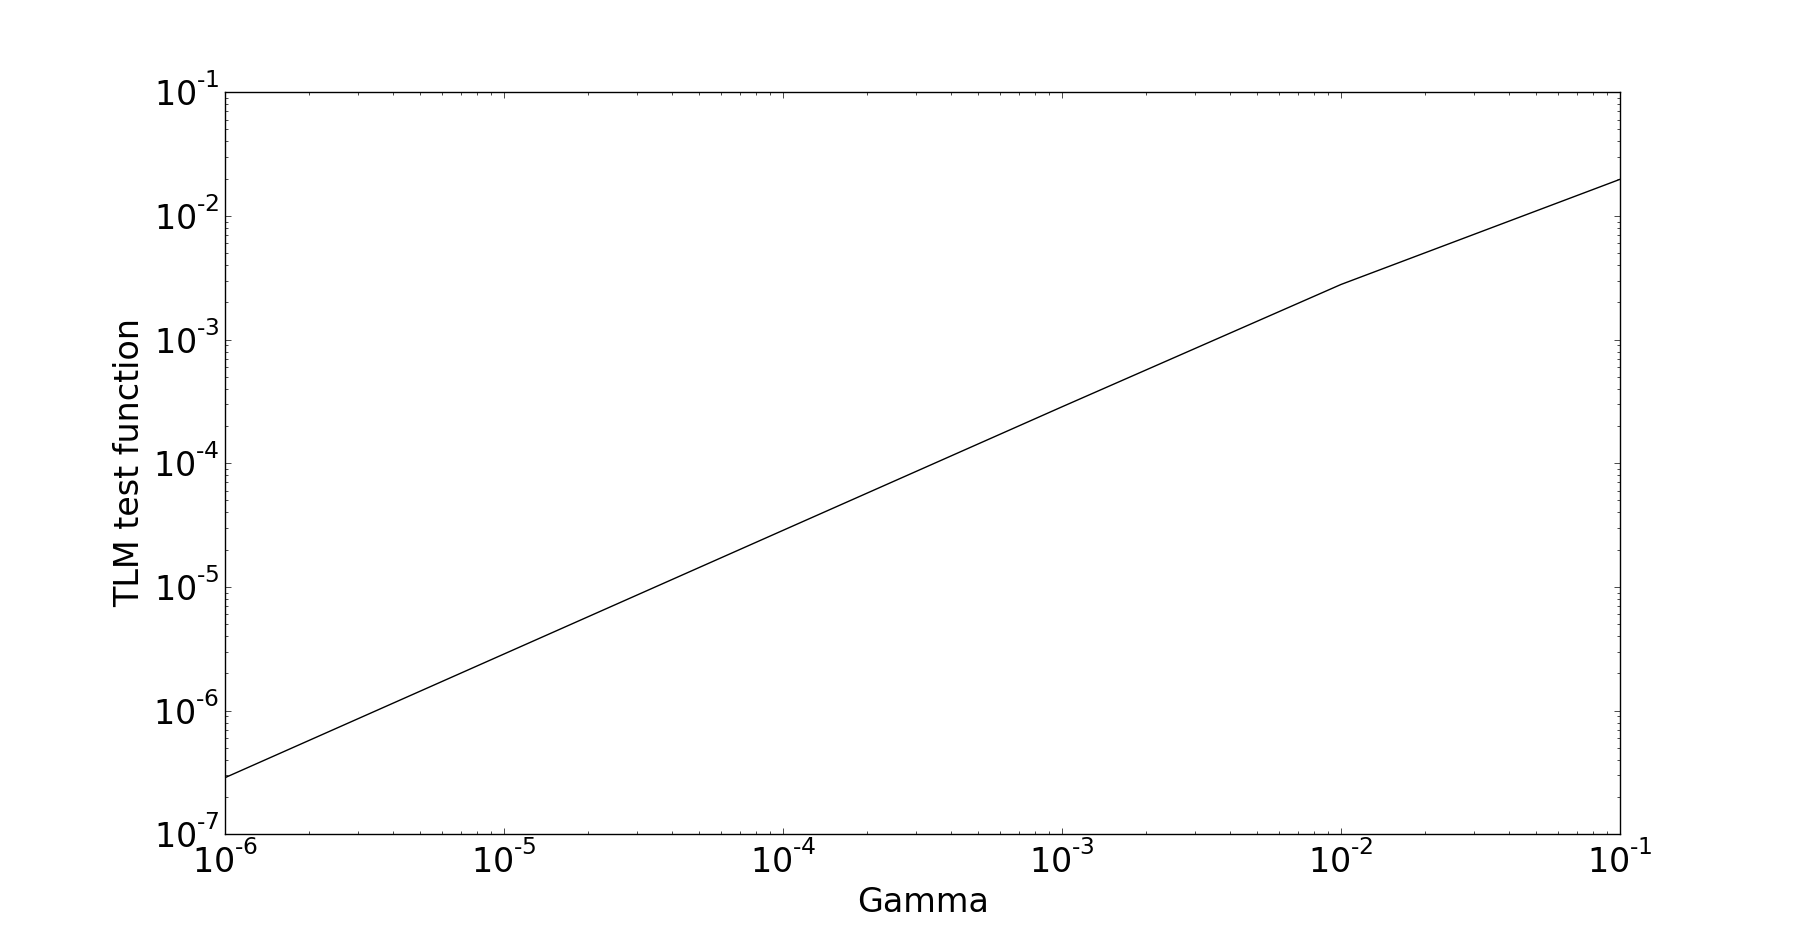
\includegraphics[width=0.6\textwidth]{testtlmer.png}
    \caption{Plot of the tangent linear model test function for DALEC2, for a TLM evolving our state 731 days forward in time and a $5\%$ perturbation, $\delta \textbf{x}_0$.}
    \label{fig:tlm}
\end{figure}

It is also useful to show how our TLM behaves over a time window to see how the error in our TLM grows as we evolve our state further forward in time. We again rearrange equation \ref{TLH} to find, 
\begin{equation}
\text{percentage error in TLM} = \begin{vmatrix} \frac{||m_{0\rightarrow i}(\mathbf{x}_0+\delta\mathbf{x}_0) - m_{0 \rightarrow i}(\mathbf{x}_0)||}{|| \mathbf{M}_{i,0}\delta\mathbf{x}_0||} - 1 \end{vmatrix} \times 100.
\end{equation}

\begin{figure}[ht]
    \centering
    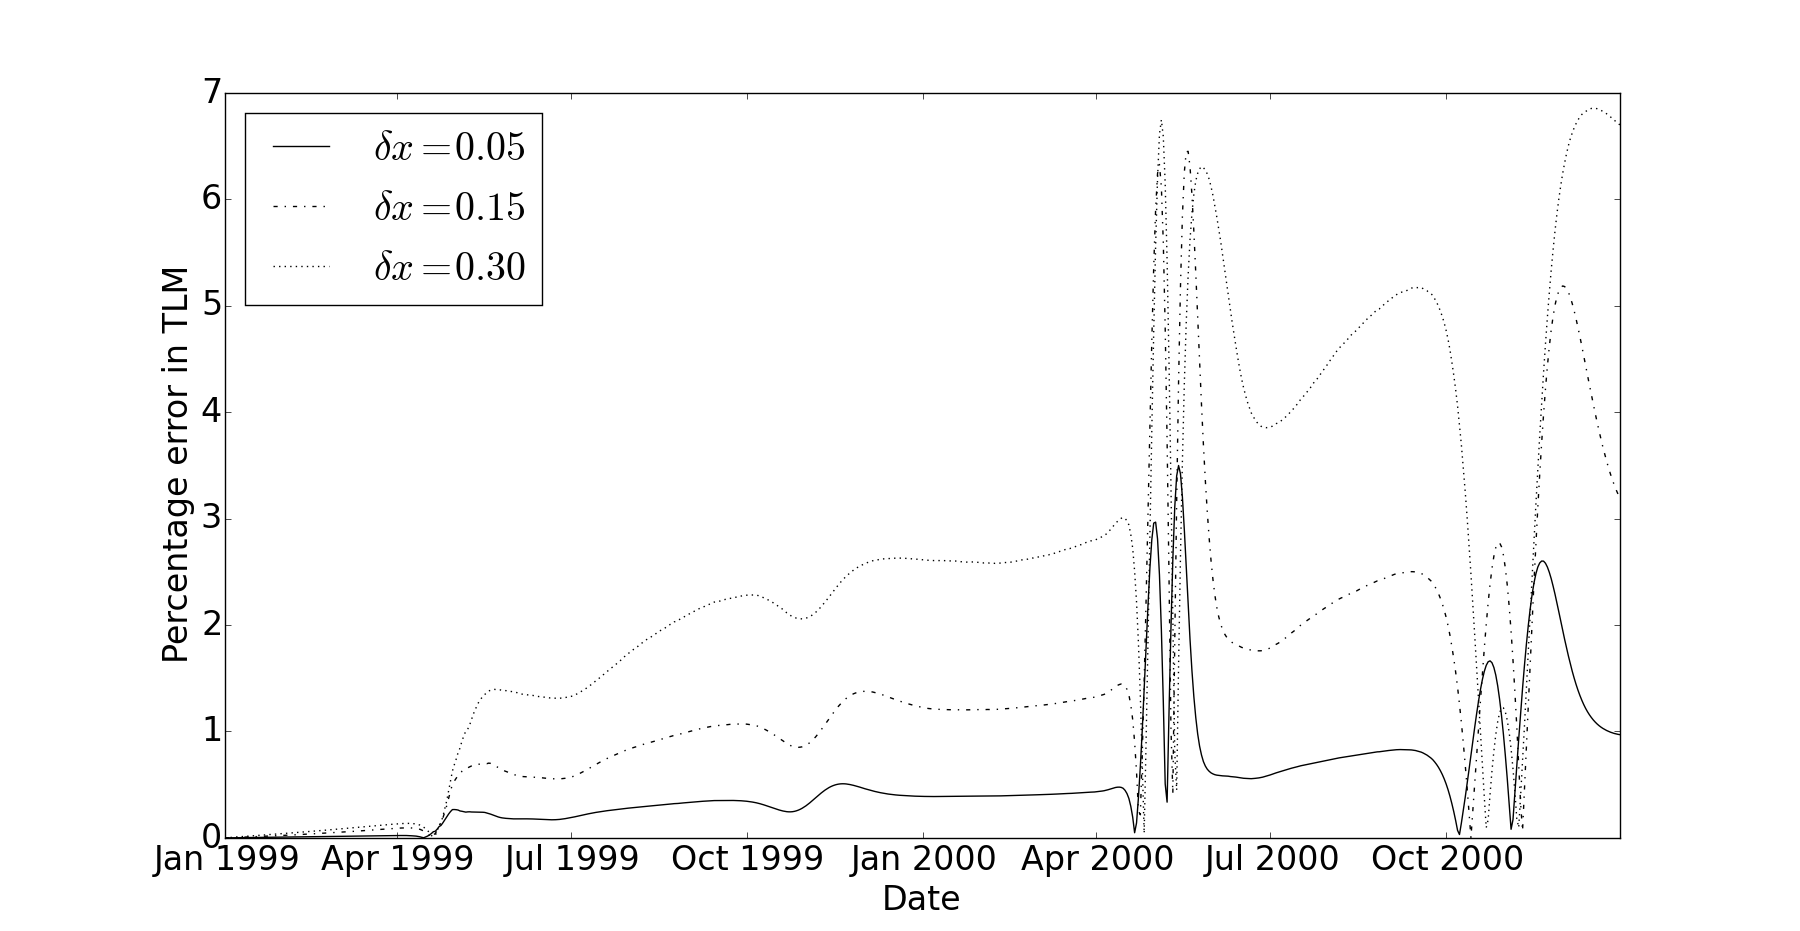
\includegraphics[width=0.6\textwidth]{tlm_error.png}
    \caption{Plot of the percentage error in our tangent linear model for DALEC2 when evolving our state forward over a period of two years with three differing values of perturbation, $\delta \textbf{x}_0$.}
    \label{fig:tlm_error}
\end{figure}

In figure \ref{fig:tlm_error} we can see that our TLM for DALEC2 performs very well after being run forward a year with less than a $3\%$ error for all values of $\delta \textbf{x}_0$. By the second year we see some peaks in our error in spring and autumn, this is where our leaf on and leaf off functions in the TLM have gone out of phase with the nonlinear DALEC2. Even at these peaks our error is still reasonable reaching a maximum at $7\%$ and then coming back to around $1\%$. For this reason we present results using a one year assimilation window in this paper. 

\subsubsection{Test of adjoint model} 

The adjoint model we have implemented for DALEC2 passes correctness tests. For our TLM $\mathbf{M}_{i,0}$ and its adjoint $\mathbf{M}_{i,0}^{T}$ we have the identity
\begin{equation}
<\mathbf{M}_{i,0}\delta\textbf{x}_0, \mathbf{M}_{i,0}\delta\textbf{x}_0> = <\delta\textbf{x}_0, \mathbf{M}_{i,0}^{T}\mathbf{M}_{i,0}\delta\textbf{x}_0>
\end{equation}
for any inner product $<, >$ and perturbation $\delta \textbf{x}_0$. This identity has been used with differing values of $\delta \textbf{x}_0$ and $i$ to show that our adjoint model is implemented correctly.

\subsubsection{Gradient test} \label{sec:testgrad}

The 4D-Var system we have developed passes tests for the gradient of the cost function. For our cost function $J$ and its gradient $\nabla J$ we can show that we have implemented $\nabla J$ correctly using the identity,
\begin{equation}
f(\alpha)=\frac{J( \textbf{x}_0 + \alpha \textbf{h}) - J(\textbf{x}_0)}{\alpha \textbf{h}^{T} \nabla J(\textbf{x}_0)} = 1 + O(\alpha),
\end{equation}
where $\textbf{h}$ is a vector of unit length. For small values of $\alpha$ not too close to machine zero we should have $f(\alpha)$ close to 1. In figure~\ref{fig:testgradcostone} we have plotted $f(\alpha)$ for a 731 day assimilation window with $\textbf{h}=\textbf{x}_0||\textbf{x}_0||^{-1}$, we can see that $f(\alpha) \rightarrow 1$ as $\alpha \rightarrow 0$, as expected.

\begin{figure}[ht]
    \centering
    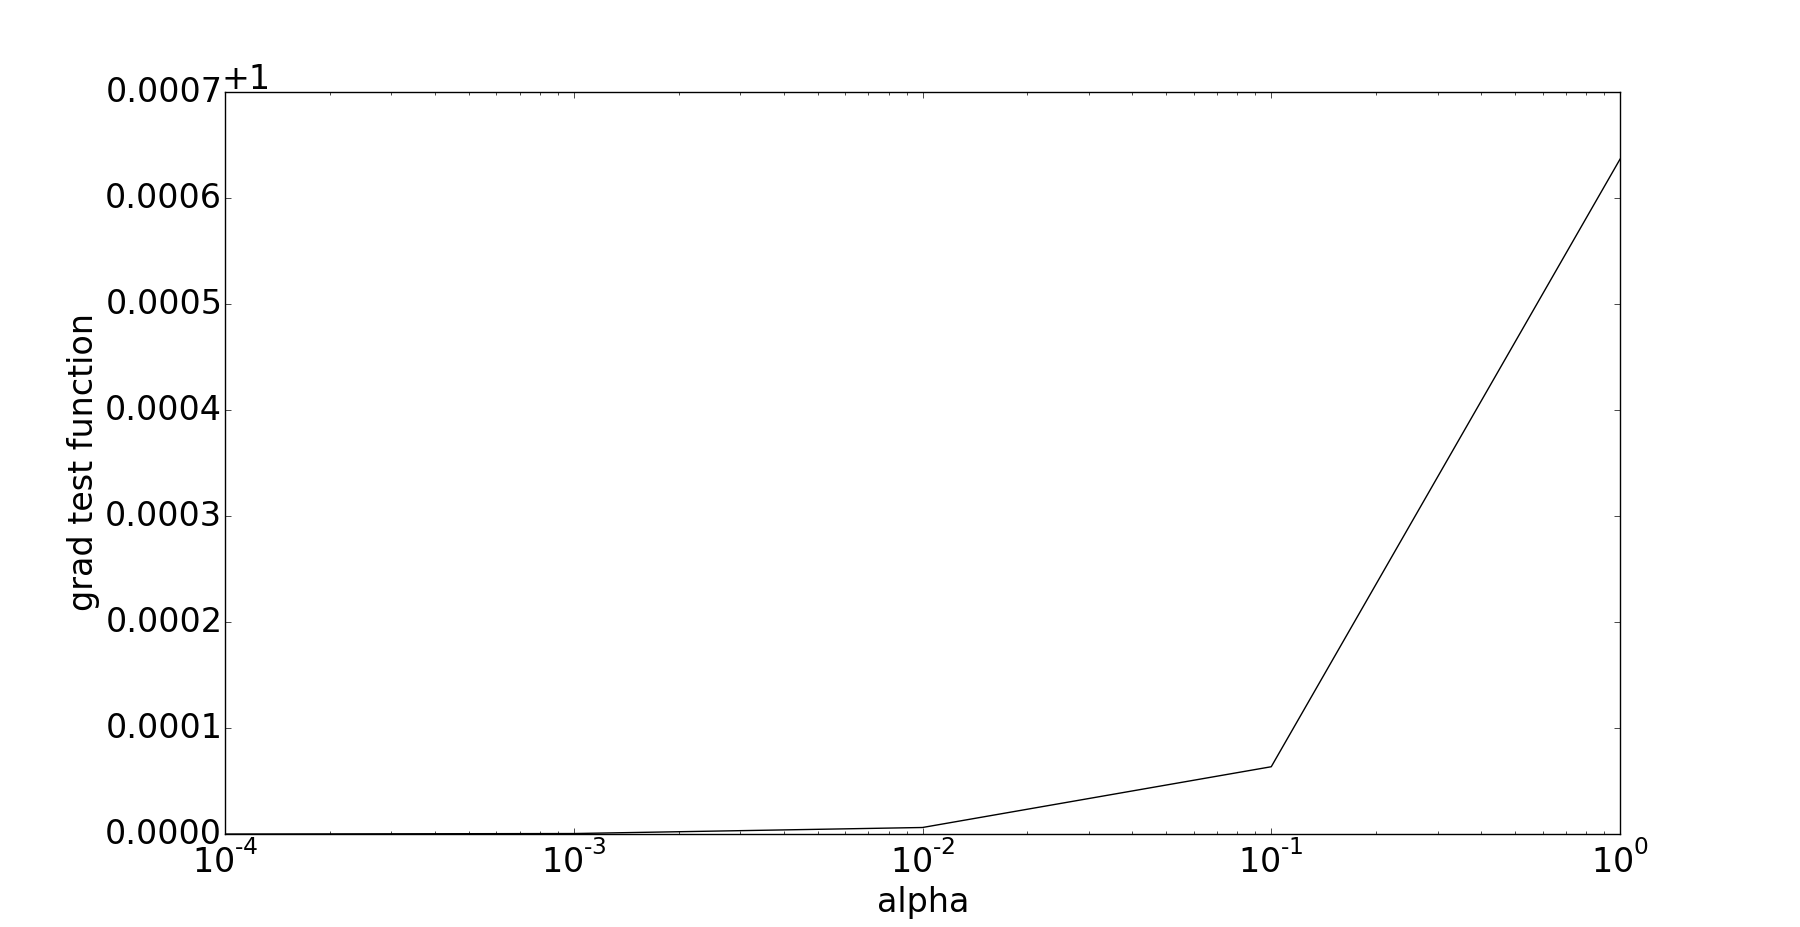
\includegraphics[width=0.6\textwidth]{gradtestone.png}
    \caption{Test of the gradient of the cost function for a 731 day assimilation window with $\textbf{h}=\textbf{x}_0||\textbf{x}_0||^{-1}$.}
    \label{fig:testgradcostone}
\end{figure}

We can also plot $|f(\alpha)-1|$, where we expect $|f(\alpha)-1| \rightarrow 0$ as $\alpha \rightarrow 0$.  In figure~\ref{fig:testgradcost} we have plotted $|f(\alpha)-1|$ for the same conditions as in figure~\ref{fig:testgradcostone}, we can see that $|f(\alpha) - 1| \rightarrow 0$ as $\alpha \rightarrow 0$, as expected (before $|f(\alpha)-1|$ gets too close to machine zero at $O(\alpha) = 10^{-5}$). This gives us confidence that the gradient of our cost function is implemented correctly.
%$\nabla J(\textbf{x}_0)||\nabla J(\textbf{x}_0)||^{-1}$. 
\begin{figure}[ht]
    \centering
    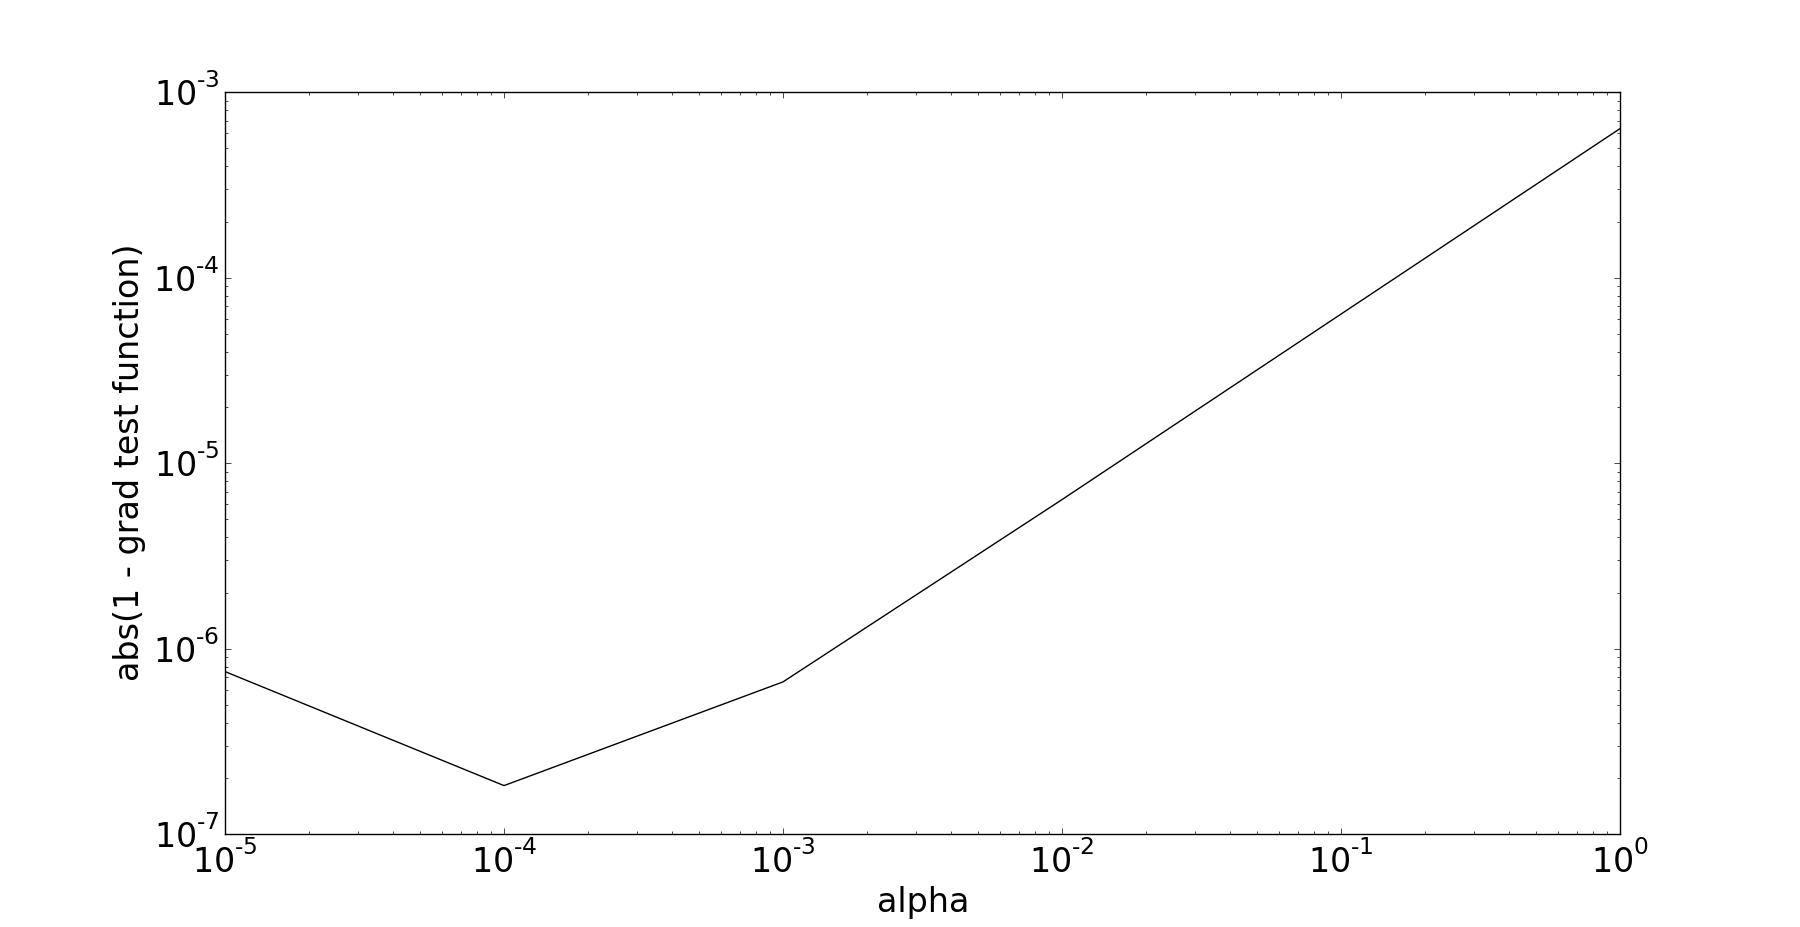
\includegraphics[width=0.6\textwidth]{testgradcost1.png}
    \caption{Test of the gradient of the cost function, $|f(\alpha) -1|$. As $\alpha \rightarrow 0$ we have $abs(1 - f(\alpha)) \rightarrow 0$ up to $O(\alpha) = 10^{-4}$ where we have gone past the precision of the computer.}
    \label{fig:testgradcost}
\end{figure}

\subsection{Including correlations in the background error covariance matrix} \label{sec:corB}

The background vector $(\textbf{x}_b)$ and its corresponding variances used in this paper were found by the University of Edinburgh using the CARbon DAta-MOdel fraMework (CARDAMOM) \citep{Exbrayat2015}. This used Harmonised World Soil Database $C_{s}$ observations as initial conditions, meteorological driving data from ERA-interim and MCMC techniques to assimilate MODIS leaf area index observations covering the Alice Holt forest over a 10 year period. So without correlations we just have the diagonal matrix of the variances, denoted as $\textbf{B}_{diag}$.

Including correlations in \textbf{B} impacts how information from assimilated observations is spread between different types of analysis variables \citep{Singh2011}. We explored a number of different methods in order to include parameter-state correlations in \textbf{B}, in this paper we present a method using a set of ecological dynamical constraints on model parameters and state variables from \citet{Bloom2015}. In this paper implementing these constraints in a Metropolis Hastings MCMC data assimilation routine are shown to improve results significantly. The constraints impose conditions on carbon pool turnover and allocation ratios, steady state proximity and growth and decay of model carbon pools.

In order to create a correlated background error covariance matrix, $\textbf{B}_{corr}$, using these constraints we first create an ensemble using the following procedure:
\begin{enumerate}
\item Draw a random state vector, $\textbf{x}_i$, from the multivariate truncated normal distribution described by our $\textbf{x}_b$, associated variances and parameter-state ranges given in table REF (in appendix).
\item Test this $\textbf{x}_i$ with the ecological dynamical constraints.
\item If $\textbf{x}_i$ passes it is added to to our ensemble, else it is discarded.
\end{enumerate}
Once we have a full ensemble we then take the covariance of the ensemble to find our $\textbf{B}_{corr}$. In figure \ref{fig:Bcorr} we have plotted the correlation matrix or normalised error covariance matrix of $\textbf{B}_{corr}$. We see that this matrix includes both positive and negative correlations between parameter and state variables, with correlations of 1 down the diagonal between variables of the same quantity as expected. The largest positive off-diagonal correlation being between $f_{lab}$ and $C_{lab}$, this makes physical sense as $f_{lab}$ is the parameter controlling the amount of GPP allocated to the labile carbon pool, $C_{lab}$.

\begin{figure}[ht]
    \centering
    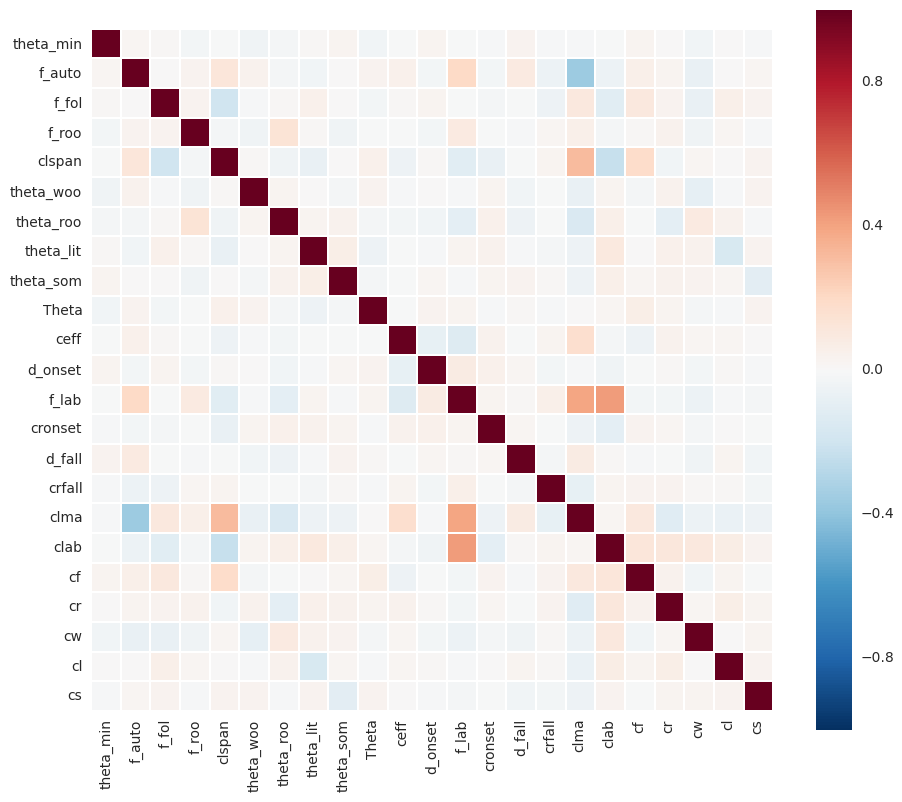
\includegraphics[width=0.5\textwidth]{b_edcNone_corrmat.png}
    \caption{Background error correlation matrix created using method in section \ref{sec:corB}}
    \label{fig:Bcorr}
\end{figure}

\subsection{Specifying serial correlations in the observational error covariance matrix} \label{sec:corR}

In this paper we use observations of NEE averaged daily. The flux towers actual sampling time is half-hourly, we take the sum over the 48 measurements made each day. We only select days where there is no missing data and over $90\% $ of observations pass quality control tests. Errors in NEE observations come from different sources such as instrument errors, sampled ecosystem structure and turbulent conditions (when we have low turbulence and limited air mixing NEE is underestimated) \citep{Papale2006}. Due to this dependance on atmospheric conditions we expect the errors in observations of NEE to be serially correlated, as the atmospheric signal itself is serially correlated \citep{Daley1992}. If we were assimilating half hourly observations of NEE we would expect stronger correlations between observation errors, as atmospheric conditions are more constant at this time scale, with correlations between observation errors getting weaker with lower frequency observations. 

In section~\ref{4dvar} we have re-written the 4D-Var cost function in equation~\ref{costfn} in order to allow the specification of serial observation error correlations in our assimilation scheme. These serial correlations are represented by the off-diagonal terms of $\hat{\mathbf{R}}$. As we do not have a practical method of estimating the serial correlation in NEE observation error we adapt the simple Gaussian model found in \citet{jarvinen1999variational} (a second order autoregressive correlation function was also tested but not presented here). Here the correlation $r$ between 2 observations at times $t_1$ and $t_2$ is given as,
\begin{equation}
r =
\begin{cases} 
      a \text{exp} \bigg[ \frac{-(t_1 - t_2)^2}{\tau^2} \bigg] + (1- a)\delta_{t_1 - t_2} & |t_1 - t_2| \leq \eta \\
      0 & \eta < |t_1 - t_2| 
   \end{cases}
   , \label{eqn:corr_fn}
\end{equation}
where $\tau$ is the e-folding time, $a$ is the correlation, $\delta$ is the Kronecker delta and $\eta$ is the cut off time after which the correlation between two observation errors is zero. We have incorporated a cut off for correlations between observation errors as we believe the correlation length scale to be quite short for our assimilated observations but also because this makes $\hat{\mathbf{R}}$ better conditioned and therefore easier to invert in the assimilation process. 

\begin{figure}[ht]
    \centering
    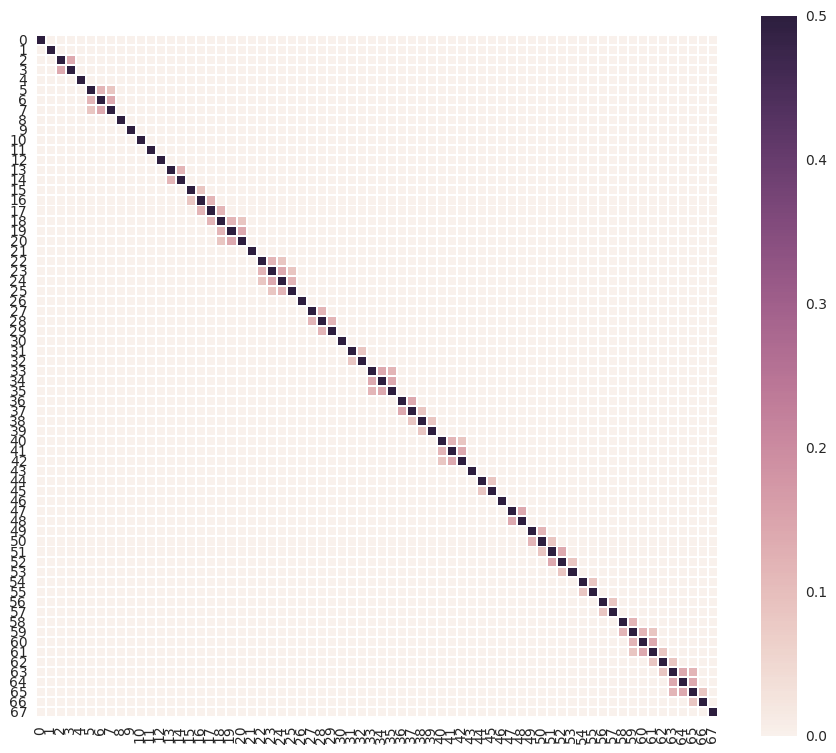
\includegraphics[width=0.5\textwidth]{b_edcr_corr_cor03_tau4_cutoff4_var05_rmat.png}
    \caption{Observation error covariance matrix created using method in section \ref{sec:corR} with $\tau = 4$, $a=0.3$ and $\eta=4$.}
    \label{fig:Rcorr}
\end{figure}

In figure~\ref{sec:corR} we show $\hat{\mathbf{R}}$ created using equation~\ref{eqn:corr_fn}, we can see that we have 67 NEE observations in our years assimilation window, these observations are obviously not all on adjacent days and this is evident in the structure of $\hat{\mathbf{R}}$. We also see the effect of the short e-folding time chosen here ($\tau=4$) giving us the desired structure as correlations are believed to be on the scale of a day. 

\subsection{Experiments} \label{sec:exps}

In this paper we will present the results of 4 experiments where we vary the representations of $\textbf{B}$ and $\hat{\mathbf{R}}$ while assimilating the same NEE observations in the years window from 1999-2000. These experiments are outlined in table~\ref{table:exps_tab} where $\textbf{B}_{diag}$ and $\hat{\mathbf{R}}_{diag}$ are the diagonal matrices of the parameter-state variances and the observations variances respectively and $\textbf{B}_{corr}$ and $\hat{\mathbf{R}}_{corr}$ are the matrices as specified in section~\ref{sec:corB} and section~\ref{sec:corR} respectively.

\begin{table}[ht] 
\begin{center}
	\begin{tabular}{| l | l | l | l | l |}
	\hline
	Experiment & $\textbf{B}_{diag}$ & $\hat{\mathbf{R}}_{diag}$ & $\textbf{B}_{corr}$ &
	$\hat{\mathbf{R}}_{corr}$ \\ \hline
	A & $\times$ & $\times$ & & \\ \hline
	B & & $\times$ & $\times$ & \\ \hline
	C & $\times$ & & & $\times$ \\ \hline
	D & & & $\times$ & $\times$ \\ 
	\hline
	\end{tabular}
	\caption{The combination of error covariance matrices used in each data assimilation experiment.}
	\label{table:exps_tab}
\end{center} 
\end{table}

In section~\ref{sec:results} we will show the results of each of the experiments and see the impact that using these different representations of $\textbf{B}$ and $\hat{\mathbf{R}}$ has on our assimilation scheme.

\section{Results} \label{sec:results}

In all the following experiments we present results when assimilating NEE observations in the period 1999-2000 from the Alice Holt flux site, other assimilation windows were also tested but are not shown here.

\subsection{Experiment A} \label{sec:expa}
In this experiment $\textbf{B}_{diag}$ and $\hat{\textbf{R}}_{diag}$ were used in our assimilation as described in section~\ref{sec:exps}. This experiment will form the standard by which the subsequent results from assimilation experiments will be judged. 

\begin{figure}[ht]
    \centering
    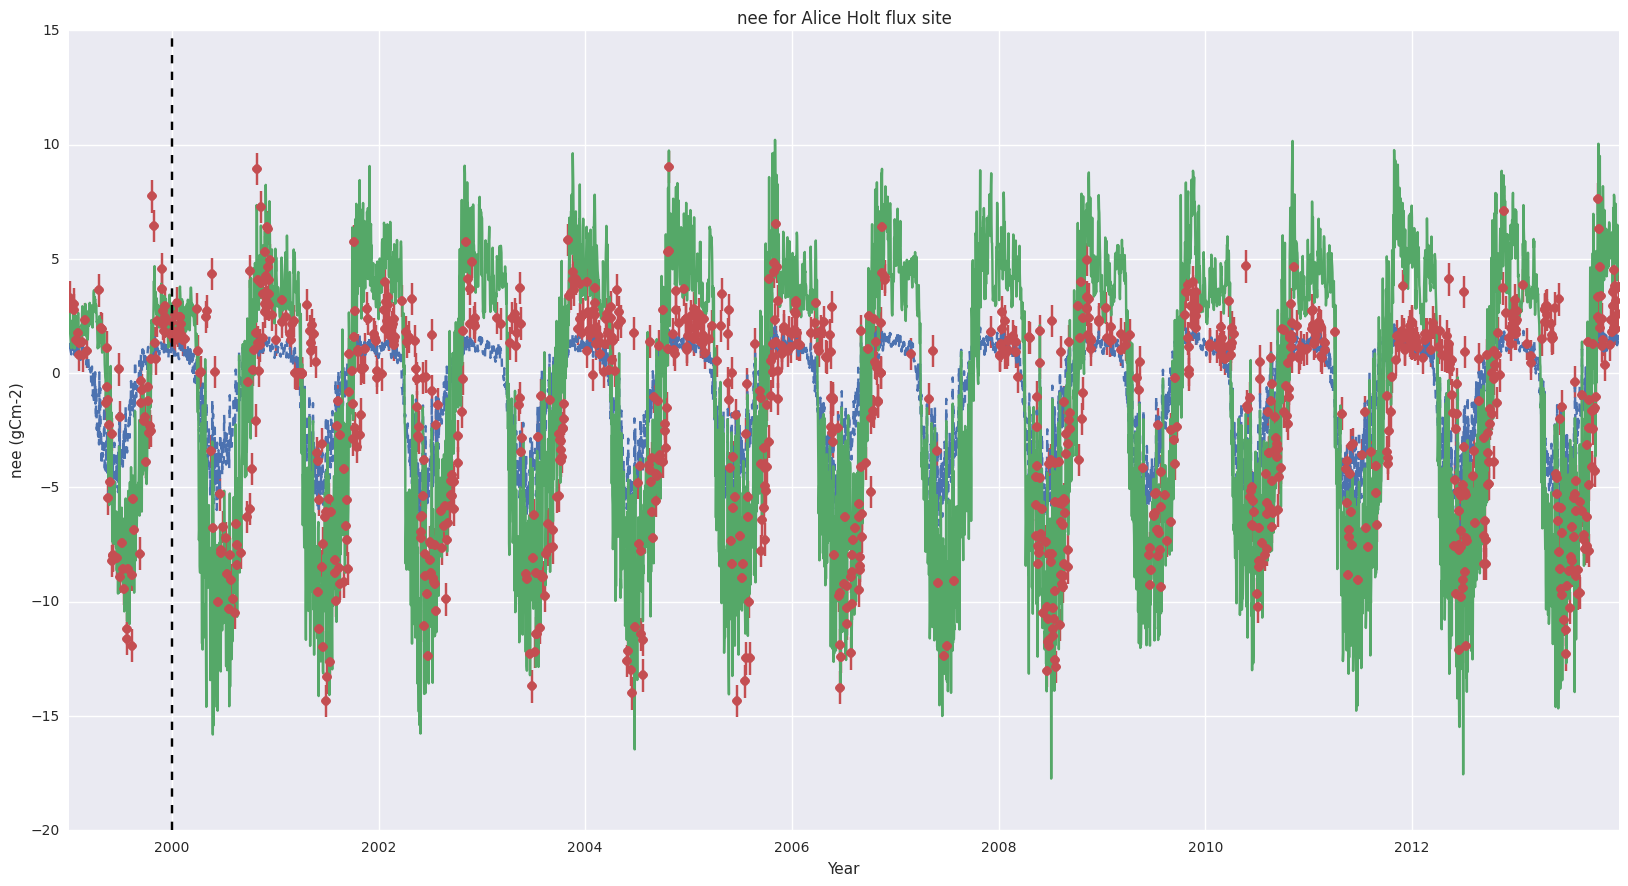
\includegraphics[width=0.6\textwidth]{bdiagNone_4dvar.png}
    \caption{One year assimilation and fourteen year forecast of Alice Holt NEE with DALEC2, blue dotted line: background model trajectory, green line: analysis and forecast after assimilation, red dots: observations from Alice Holt flux site with error bars. Number of function evaluations needed for minimisation to converge: 571.}
    \label{fig:4dvardiagBR}
\end{figure}

In figur~\ref{fig:4dvardiagBR} we have plotted assimilation and forecast results for NEE. We can see that our analysis trajectory (green line) fits well with the observations during the the assimilation window (1999-2000) and then diverges in the forecast (2000-2014). One reason for this is that our analysis is being over constrained by the observations and under constrained by the background. Using a diagonal background error covariance matrix ($\textbf{B}_{diag}$) we are not adding much background information to our system and therefore the observations dominate and result in the over fitting of our analysis to the assimilated observations of NEE.

\begin{figure}[ht]
    \centering
    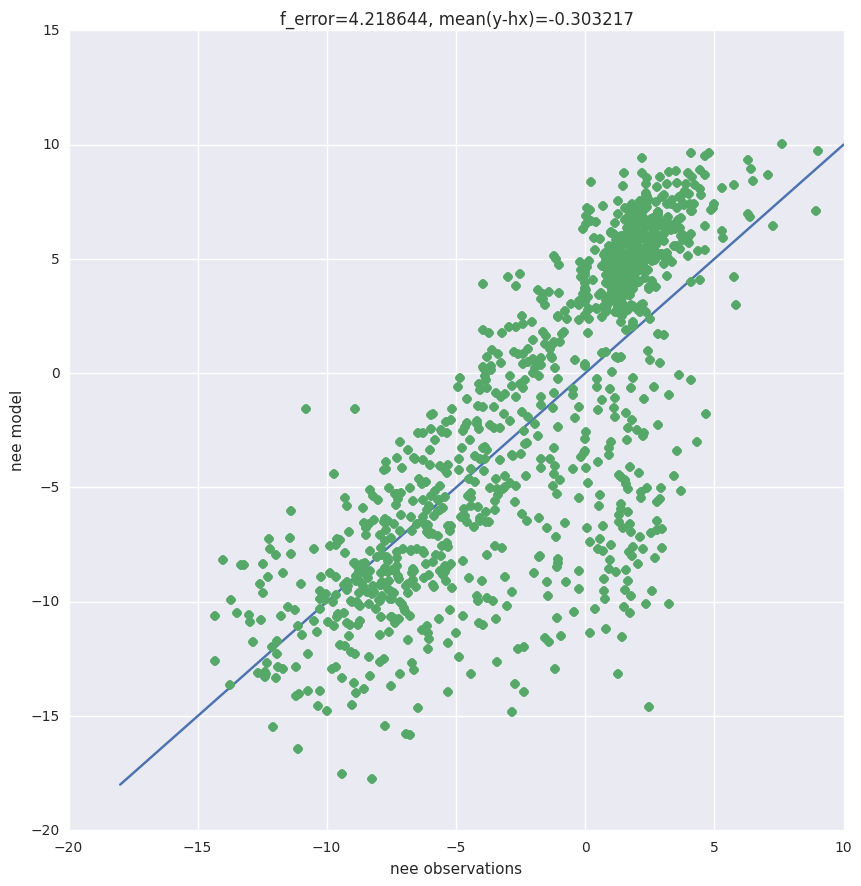
\includegraphics[width=0.3\textwidth]{bdiagNone_forecast_scatter.png}
    \caption{Forecast scatter plot of modelled NEE vs. observations for 2000-2014 (green dots), forecasted NEE has a root-mean squared error of $4.22 \text{gCm}^{-2}$ between model and observations. Blue line represents 1-1 line where all green dots would lie if the model predicted the observations perfectly.}
    \label{fig:forecastscatBR}
\end{figure}

To see how well our forecast performs after assimilation we show a scatter plot of modelled NEE against observed NEE in figure~\ref{fig:forecastscatBR}. Here we have a Root-Mean-Square Error (RMSE) of $4.22 \text{gCm}^{-2}$ and a bias of $-0.3 \text{gCm}^{-2}$ for our forecast of NEE, whereas our analysis (1999-2000) has a RMSE of $1.36 \text{gCm}^{-2}$ and a bias of $-0.03 \text{gCm}^{-2}$. The background trajectory meanwhile has a RMSE of $3.86 \text{gCm}^{-2}$ and a bias of $-1.60 \text{gCm}^{-2}$ in the analysis window (1999-2000) and the same RMSE of $3.86 \text{gCm}^{-2}$ but a bias of $-1.36 \text{gCm}^{-2}$ during the forecast period (2000-2014). So we see that although using $\textbf{B}_{diag}$ and $\hat{\textbf{R}}_{diag}$ in our assimilation has considerably reduced the RMSE in our analysis period, it has also increased the RMSE in our forecast of NEE. However it has reduced the bias in the models forecast considerably from $-1.36 \text{gCm}^{-2}$ to $-0.3 \text{gCm}^{-2}$. The bias in our background comes from a constant under prediction of the more extreme negative values of NEE and this leads to considerably worse results than our analysis and its forecast for total forest carbon uptake. 

{\color{red} **Maybe include something about the estimated reduction in error for parameter and state variables using the diagonal terms of \textbf{B} and \textbf{A} (analysis error covariance matrix). How best to compare and present these?}

\subsection{Experiment B} \label{sec:expb}

Here $\textbf{B}_{corr}$ (as defined in section~\ref{sec:corB}) and $\hat{\textbf{R}}_{diag}$ are used in our assimilation. In figure~\ref{fig:4dvaredcBR} we can see that our forecast performs considerably better than in experiment A and indeed from figure~\ref{fig:forecastscatedcBR} we see that our forecasts RMSE has almost halved (now $2.56 \text{gCm}^{-2}$) with a reduction in bias also, now $-0.2 \text{gCm}^{-2}$. In comparison using $\textbf{B}_{corr}$ in our assimilation slightly degrades the fit for our analysis (1999-2000), with a RMSE of $1.42 \text{gCm}^{-2}$ and a bias of $-0.04 \text{gCm}^{-2}$, this is because our assimilation scheme is now more constrained by the background than in experiment A. Therefore using $\textbf{B}_{corr}$ in our assimilation reduces the problem of overfitting to our assimilated observations of NEE as seen in experiment A. Another improvement made by using $\textbf{B}_{corr}$ in our assimilation is that our minimisation routine converges to a solution more quickly, taking 218 fewer function iterations than experiment A to converge. 

\begin{figure}[ht]
    \centering
    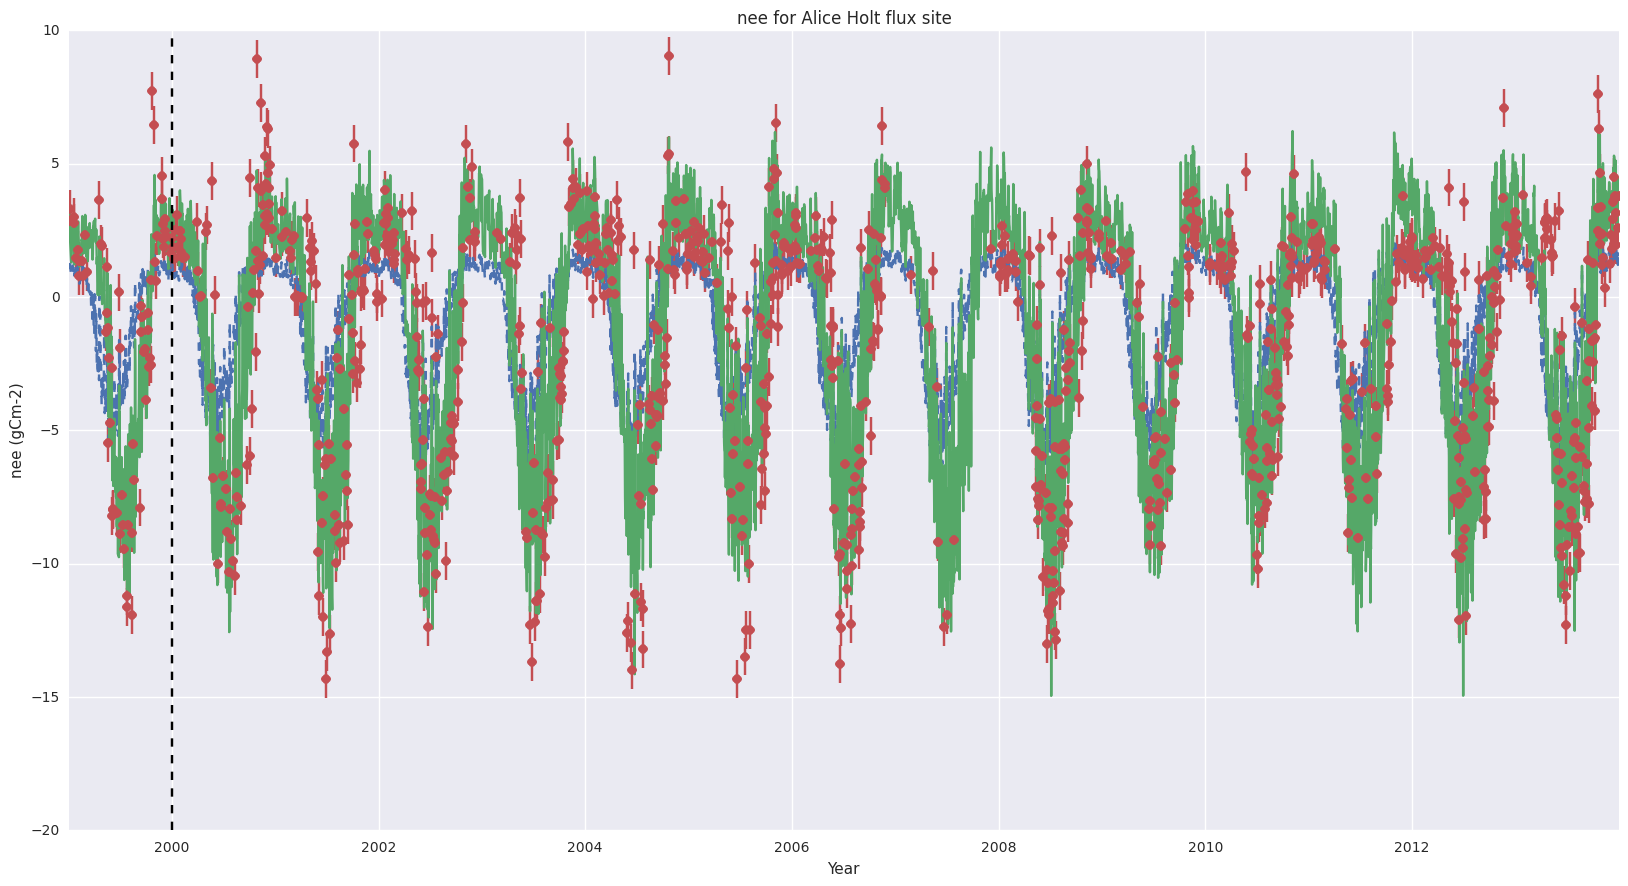
\includegraphics[width=0.6\textwidth]{b_edcNone_4dvar.png}
    \caption{One year assimilation and fourteen year forecast of Alice Holt NEE with DALEC2, blue dotted line: background model trajectory, green line: analysis and forecast after assimilation, red dots: observations from Alice Holt flux site with error bars.Number of function evaluations needed for minimisation to converge: 353.}
    \label{fig:4dvaredcBR}
\end{figure}

\begin{figure}[ht]
    \centering
    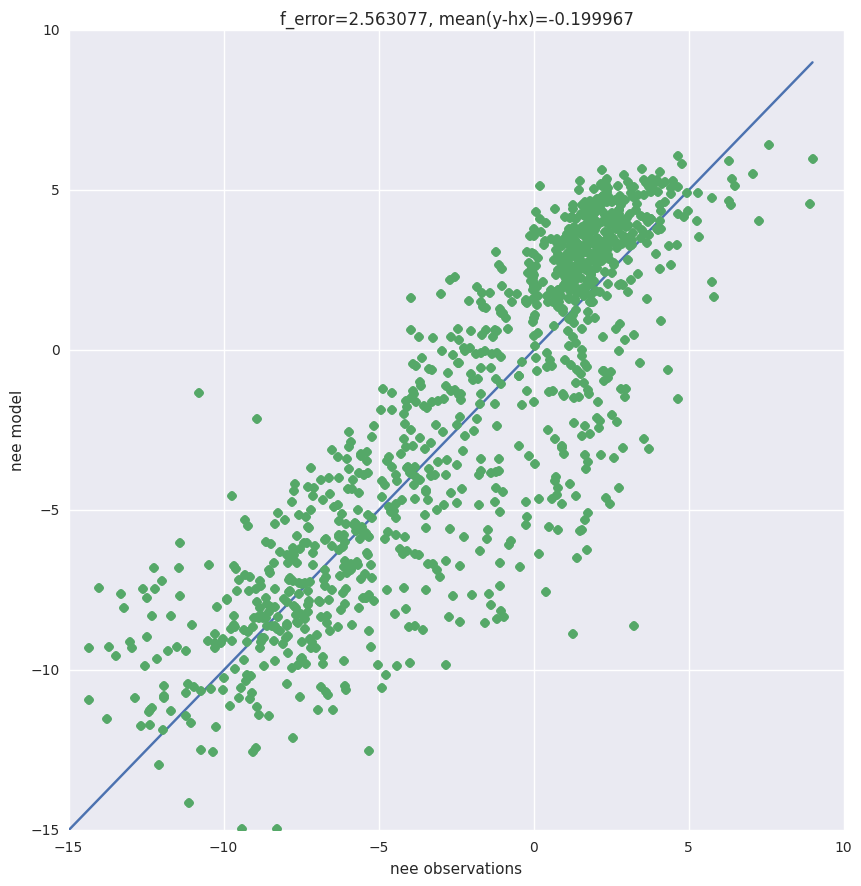
\includegraphics[width=0.3\textwidth]{b_edcNone_forecast_scatter.png}
    \caption{Forecast scatter plot of modelled NEE vs. observations for 2000-2014 (green dots), forecasted NEE has a root-mean squared error of $2.56 \text{gCm}^{-2}$ between model and observations. Blue line represents 1-1 line where all green dots would lie if the model predicted the observations perfectly.}
    \label{fig:forecastscatedcBR}
\end{figure}

\subsection{Experiment C} \label{sec:expc}

Here we use $\textbf{B}_{diag}$ and $\hat{\textbf{R}}_{corr}$ (as defined in section~\ref{sec:corR}) in our assimilation. We can see from figure~\ref{fig:4dvardiagBcorR} that our results look similar to those in section~\ref{sec:expa} however there are some differences. Using $\hat{\textbf{R}}_{corr}$ in our assimilation has also reduced our minimisation routines convergence time, taking 127 less function iterations to converge than experiment A. We also have a slight reduction in RMSE for our forecast (now $4.09 \text{gCm}^{-2}$) from experiment A. As in experiment B our analysis gets slightly worse as using $\hat{\textbf{R}}_{corr}$ acts to reduce the overfitting of the analysis to the assimilated observations. The changes seen when using $\hat{\textbf{R}}_{corr}$ in our assimilation are less extreme than when using $\textbf{B}_{corr}$ as the correlations we have specified in $\hat{\textbf{R}}_{corr}$ are quite small, we have therefore added less information to our system when using $\hat{\textbf{R}}_{corr}$ in our assimilation. We would expect the effect to be larger if using a model with a half-hourly time step assimilating half-hourly observations of NEE as we would then have much stronger correlations in $\hat{\textbf{R}}_{corr}$ (as discussed in section~\ref{sec:corR}). We also expect that specifying these correlations in  $\hat{\textbf{R}}$ will help when assimilating other less frequently sampled data streams along with NEE as the serial correlations reduce the weight given to the mean of the observations and also reduce the information content of the data streams with more observations \citep{jarvinen1999variational, Daley1992}.

\begin{figure}[ht]
    \centering
    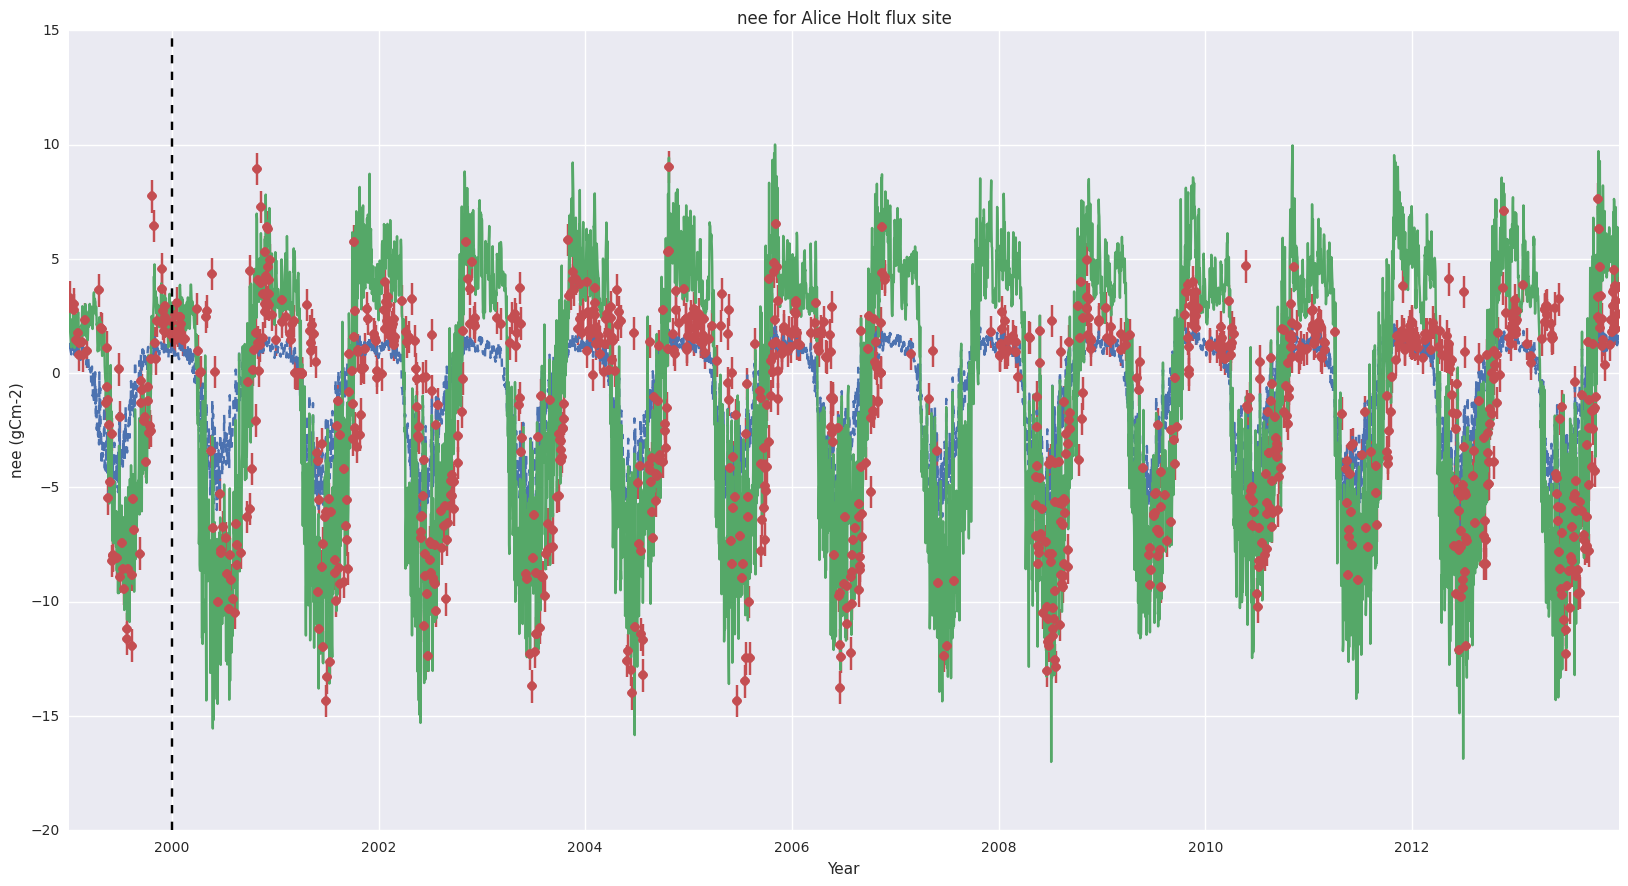
\includegraphics[width=0.6\textwidth]{bdiagr_corr_cor03_tau4_cutoff4_var05_4dvar.png}
    \caption{One year assimilation and fourteen year forecast of Alice Holt NEE with DALEC2, blue dotted line: background model trajectory, green line: analysis and forecast after assimilation, red dots: observations from Alice Holt flux site with error bars. Number of function evaluations needed for minimisation to converge: 444.}
    \label{fig:4dvardiagBcorR}
\end{figure}

\begin{figure}[ht]
    \centering
    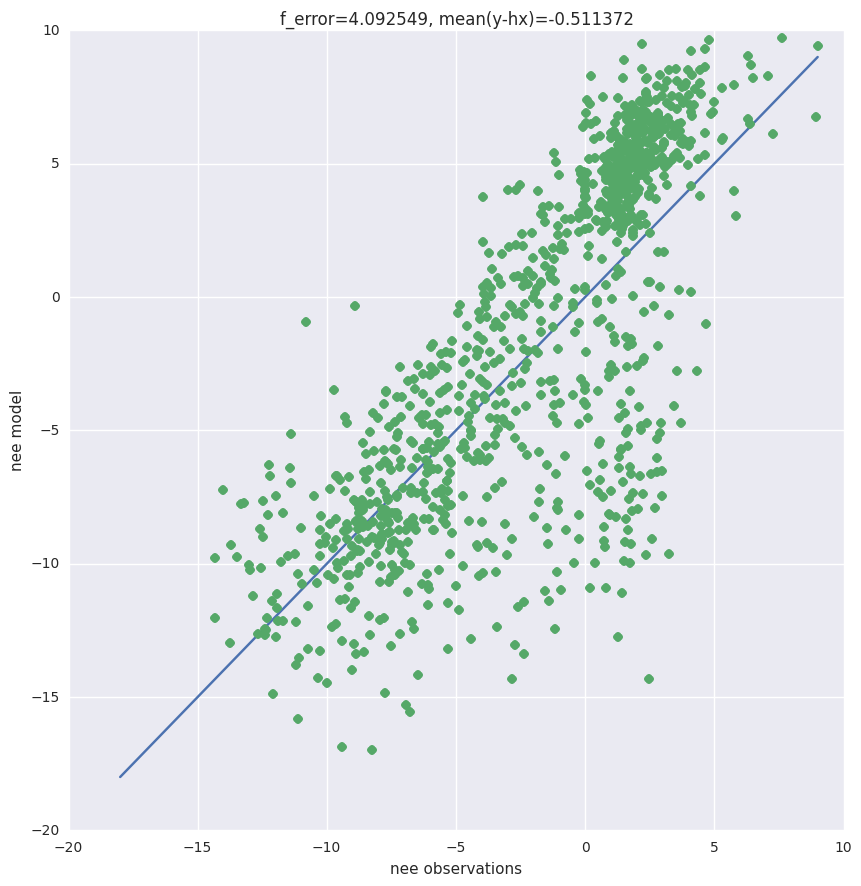
\includegraphics[width=0.3\textwidth]{bdiagr_corr_cor03_tau4_cutoff4_var05_forecast_scatter.png}
    \caption{Forecast scatter plot of modelled NEE vs. observations for 2000-2014 (green dots), forecasted NEE has a root-mean squared error of $4.09 \text{gCm}^{-2}$ between model and observations. Blue line represents 1-1 line where all green dots would lie if the model predicted the observations perfectly.}
    \label{fig:forecastscatBR}
\end{figure}

\subsection{Experiment D}

In the final experiment we use $\textbf{B}_{corr}$ and $\hat{\textbf{R}}_{corr}$ in our assimilation. From figure~\ref{fig:4dvaredcBcorR} we see that using both correlated matrices gives similar results as experiment B when $\textbf{B}_{corr}$ is used with $\hat{\textbf{R}}_{diag}$. However using $\hat{\textbf{R}}_{corr}$ in addition to $\textbf{B}_{corr}$ provides similar improvements as in experiment C. The number of function evaluations taken for our minimisation routine to converge is the lowest yet at 316. Also our forecast RMSE is reduced again still from results in experiment B to $2.38 \text{gCm}^{-2}$. Using both matrices appears to combine the beneficial effects described in both section~\ref{sec:expb} and section~\ref{sec:expc}.
 
From our results in experiment D the forecasted (2000-2014) total carbon uptake for our research site is $5.04\times 10^6 \text{kgC}$ ({\color{red} try to find better units for this?}). In comparison our less accurate results from experiment A (using $\textbf{B}_{diag}$ and $\hat{\textbf{R}}_{diag}$) predict a total carbon uptake of $5.26 \times 10^6\text{kgC}$, a difference of $2.25 \times 10^5\text{kgC}$. This is quite a substantial difference as we are considering the carbon uptake of a small ($\sim 0.93\text{km}^2$) research site only.

 \begin{figure}[ht]
    \centering
    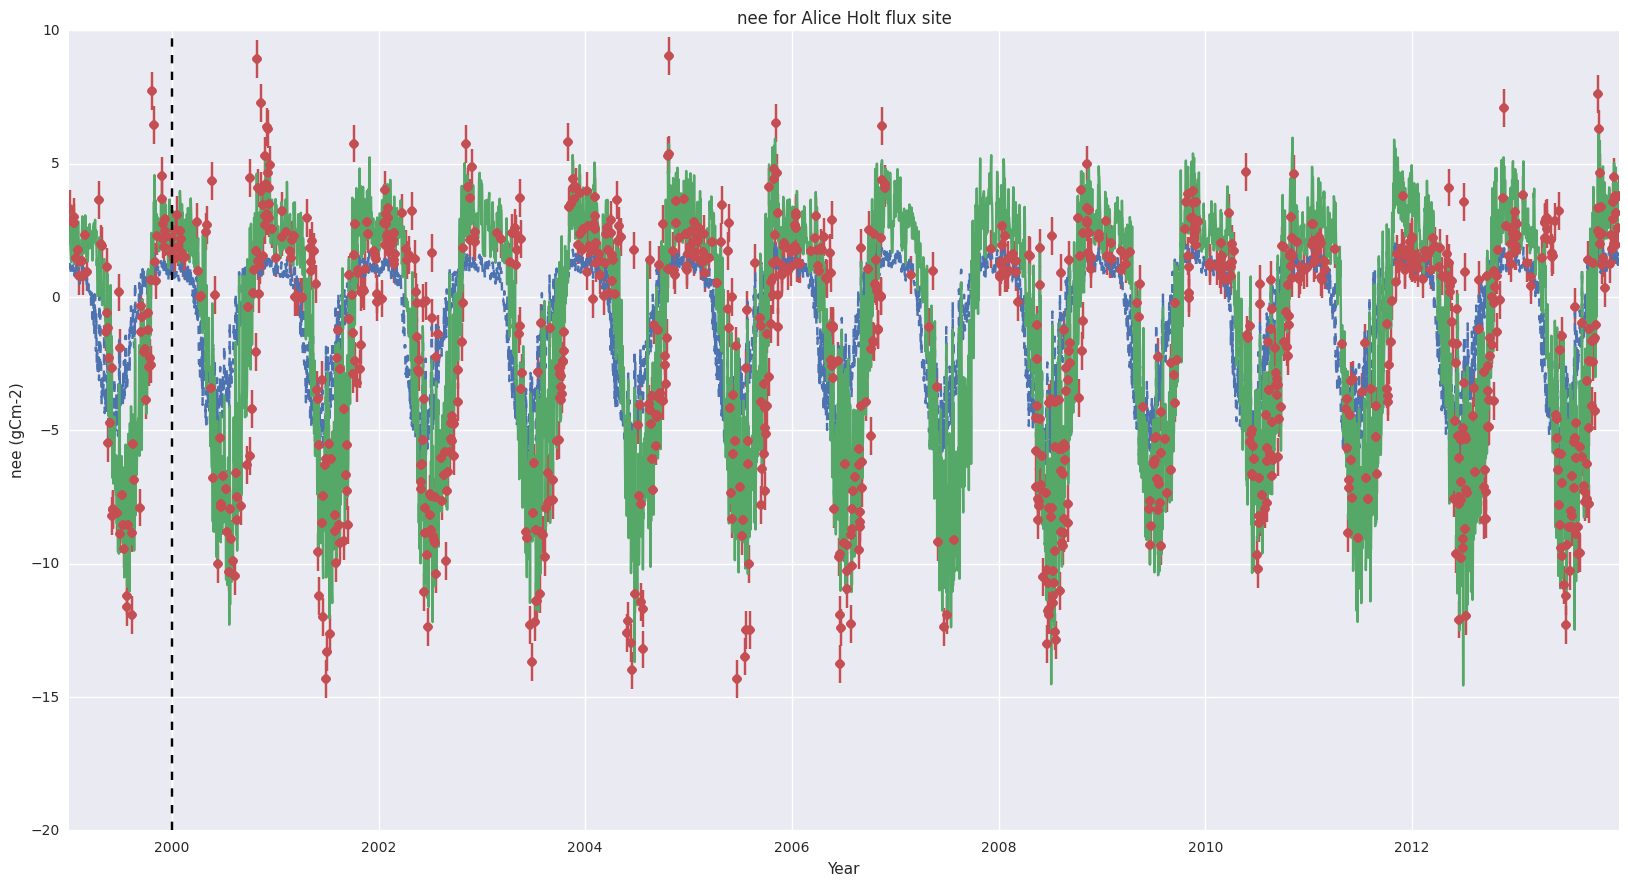
\includegraphics[width=0.6\textwidth]{b_edcr_corr_cor03_tau4_cutoff4_var05_4dvar.png}
    \caption{One year assimilation and fourteen year forecast of Alice Holt NEE with DALEC2, blue dotted line: background model trajectory, green line: analysis and forecast after assimilation, red dots: observations from Alice Holt flux site with error bars. Number of function evaluations needed for minimisation to converge: 316.}
    \label{fig:4dvaredcBcorR}
\end{figure}

\begin{figure}[ht]
    \centering
    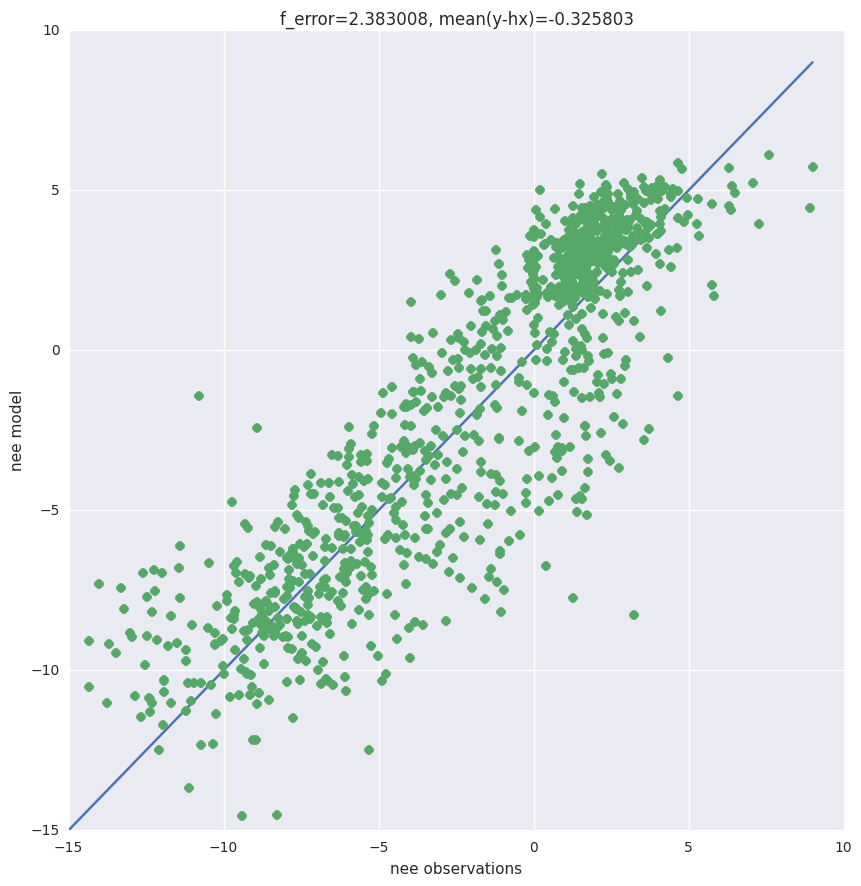
\includegraphics[width=0.3\textwidth]{b_edcr_corr_cor03_tau4_cutoff4_var05_forecast_scatter.png}
    \caption{Forecast scatter plot of modelled NEE vs. observations for 2000-2014 (green dots), forecasted NEE has a root-mean squared error of $2.38 \text{gCm}^{-2}$ between model and observations. Blue line represents 1-1 line where all green dots would lie if the model predicted the observations perfectly.}
    \label{fig:forecastscatedcBcorR}
\end{figure}


\begin{table}[ht] 
\begin{center}
	\begin{tabular}{| l | l | l | l | l |}
	\hline
	Experiment & \pbox{5cm}{Analysis RMSE \\ $( \text{gCm}^{-2})$} & \pbox{5cm}{Forecast RMSE \\ $( \text{gCm}^{-2})$} & \pbox{5cm}{Forecast bias \\ $( \text{gCm}^{-2})$} & \pbox{5cm}{Minimisation function \\ evaluations} \\ \hline
	Background & $3.86$ & $3.86$ & $-1.36$ & $n/a$ \\ \hline
	A & $1.36$ & $4.22$ & $-0.30$ & $571$ \\ \hline
	B & $1.42$ & $2.56$ & $-0.20$ & $353$  \\ \hline
	C & $1.37$ & $4.09$ & $-0.51$ & $444$ \\ \hline
	D & $1.43$ & $2.38$ & $-0.33$ & $316$ \\ 
	\hline
	\end{tabular}
	\caption{Results from experiments outlined in section  \ref{sec:exps}}
	\label{table:exps_tab}
\end{center} 
\end{table}


\section{Discussion}

\begin{itemize}
\item In this paper we have implemented the DALEC2 functional ecology model in a 4D-Var data assimilation scheme, building an adjoint of the DALEC2 model and applying rigorous tests to our scheme. Using 4D-Var can provide much quicker assimilation results than MCMC techniques as we have knowledge of the derivative of the model, however we do also assume that the problem is Gaussian whereas MCMC techniques do not. We have shown that 4D-Var is a valid tool for improving the DALEC2 model estimate of NEE.

\item We then considered the nature of background and observational errors. The effect of specifying parameter-state correlations in our background information and serial correlations between our observation errors was explored.

\item The technique presented here to specify ${\mathbf{B}}_{corr}$ has been shown to significantly improve forecasts of NEE. Other techniques were also tested (not presented here) to create a correlated $\textbf{B}$, one of which added correlations to $\textbf{B}$ using the DALEC2 model. Here we evolved an ensemble of state vectors over the length of the chosen assimilation window, then taking the covariance of the evolved ensemble. This gave us a \textbf{B} with parameter-state and state-state correlations, but no parameter-parameter correlations as the parameters are not updated by the model. Using the $\textbf{B}$ created with this method also improved assimilation results considerably in some cases. Many different tests were run using different background vectors and variances and it was found that specifying some form of correlations in $\textbf{B}$ always made some improvement to the results of our assimilation.

\item Here the $\hat{\mathbf{R}}_{corr}$ used in our experiments has improved our forecast of NEE, however many other choices of $\hat{\mathbf{R}}_{corr}$ tested for this paper degraded the forecast. This is probably due to specifying unrealistic correlations and suggests a more diagnostic approach is needed for the calculation of serial correlations in $\hat{\mathbf{R}}$. One option would be to adapt the Deroziers diagnostic \citep{desroziers2005diagnosis}, which has been used successfully in NWP for diagnosing observation error correlations for observations taken at the same time, and extending this technique to diagnose serial correlations.

\item Specifying serial correlations also allows us to address the issues discussed by \citet{richardson2010estimating}, that when assimilating multiple data streams more frequently sampled observation types (such as NEE) have much more impact on the assimilation than data streams sampled less frequently. Specifying serial correlations between observations of the same type has the effect of reducing the weight given to the mean of the observations \citep{jarvinen1999variational}, thus allowing less frequent data streams to have more impact on the assimilation. 

Using the form of $\hat{\mathbf{R}}$ given in this paper for specifying serial correlations will also allow us to specify serial correlations between different observation types. When running the model with a day-night time step this will allow us to build in the type of correlations investigated by \citet{Baldocchi2015} between ecosystem respiration and canopy photosynthesis.

\item We have also seen an improvement in convergence times for our minimisation routine when specifying correlations in our $\textbf{B}$ and $\hat{\mathbf{R}}$ matrices, this has been the case in most other tests not presented here. This is due to the correlated matrices constraining the assimilation more and making the problem less ill-posed.
\end{itemize} 

\section{Conclusion}

\begin{itemize}
\item 4DVar is a valid tool for improving the DALEC2 model estimate of NEE.
\item Including correlations in the background error covariance matrix improves our forecast after assimilation (sometimes greatly) in comparison to using a diagonal representation of $\textbf{B}$.
\item Specifying serial correlations between observation errors in $\hat{\textbf{R}}$ can improve our forecast, however more work is needed to find a method for diagnosing these correlations.
\end{itemize}


\begin{sidewaysfigure}
    \centering
    \begin{subfigure}[b]{0.48\textwidth}
        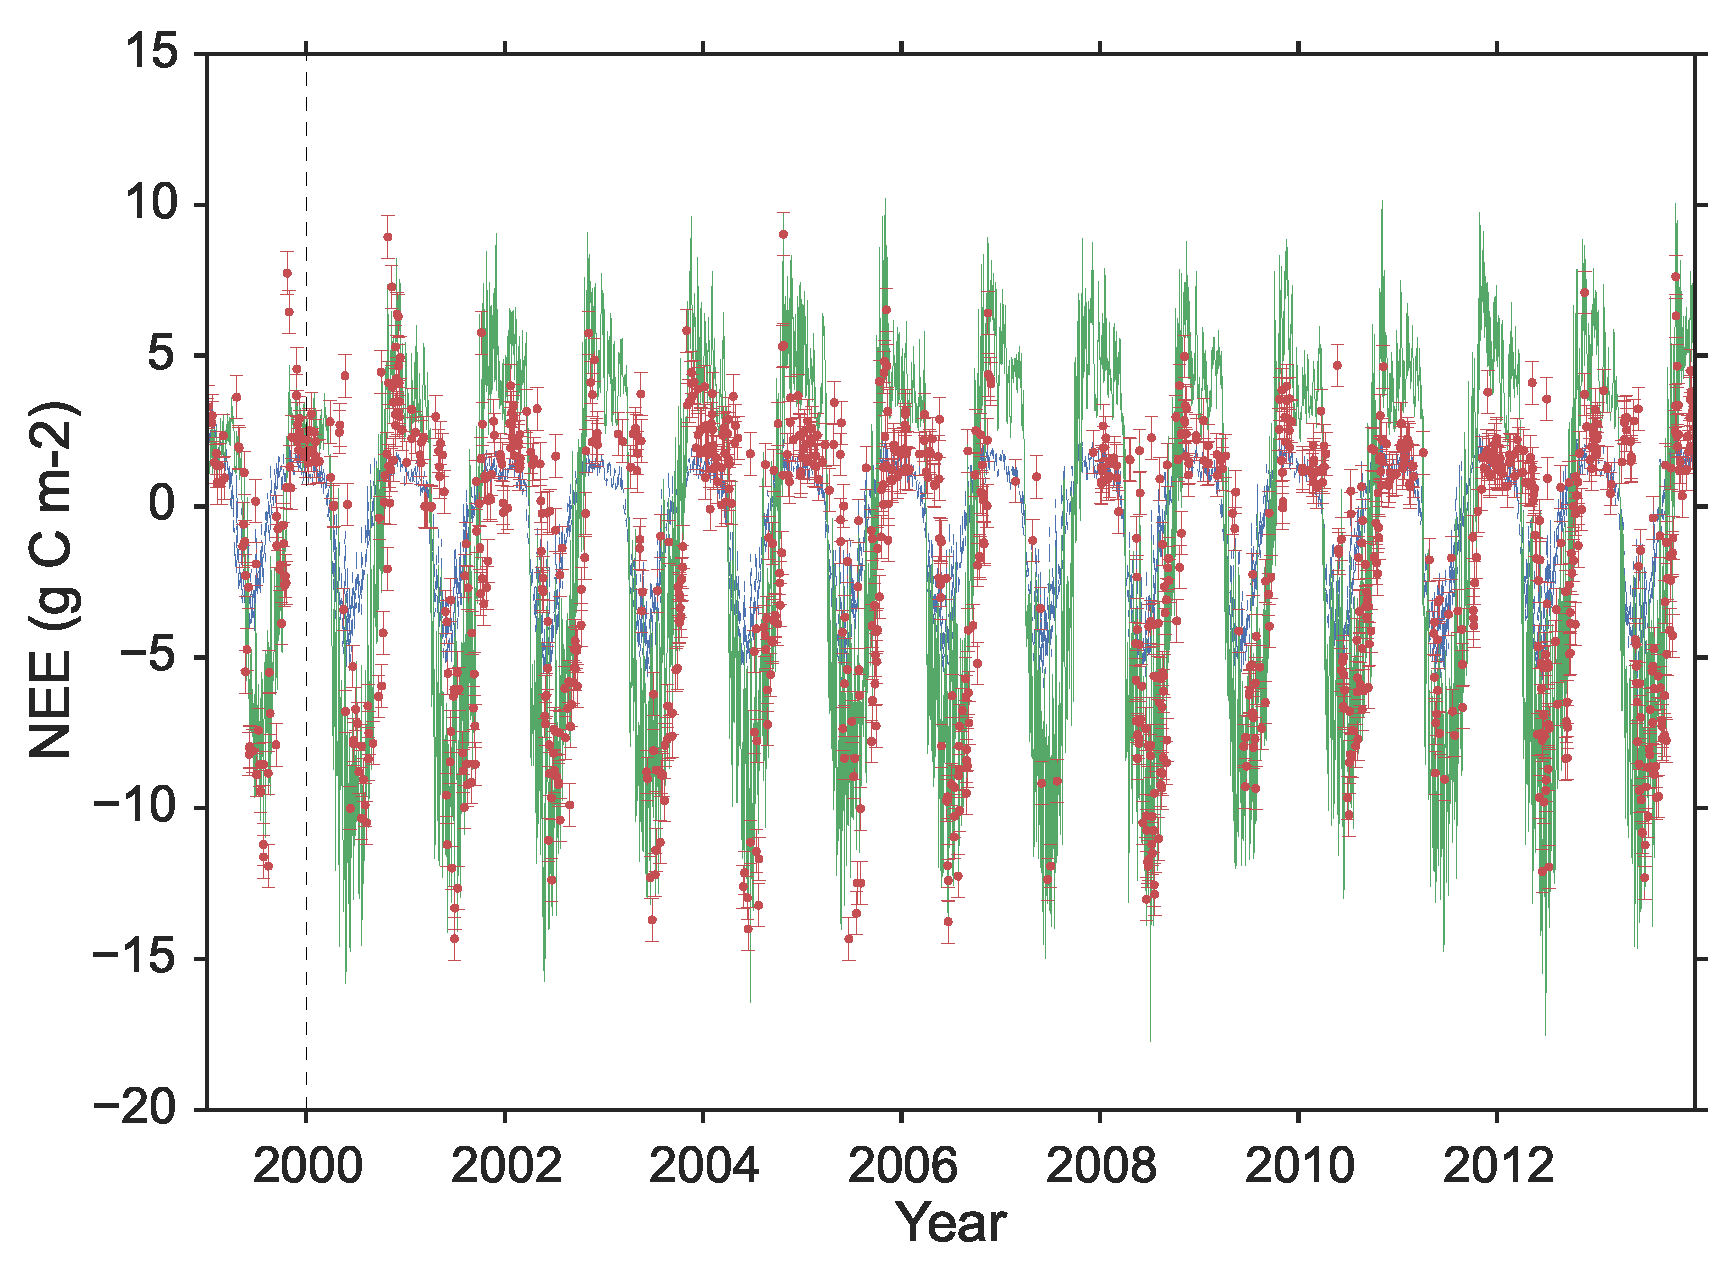
\includegraphics[width=\textwidth]{A4dvar.eps}
        \caption{Experiment A}
        \label{fig:gull}
    \end{subfigure}
    \begin{subfigure}[b]{0.48\textwidth}
        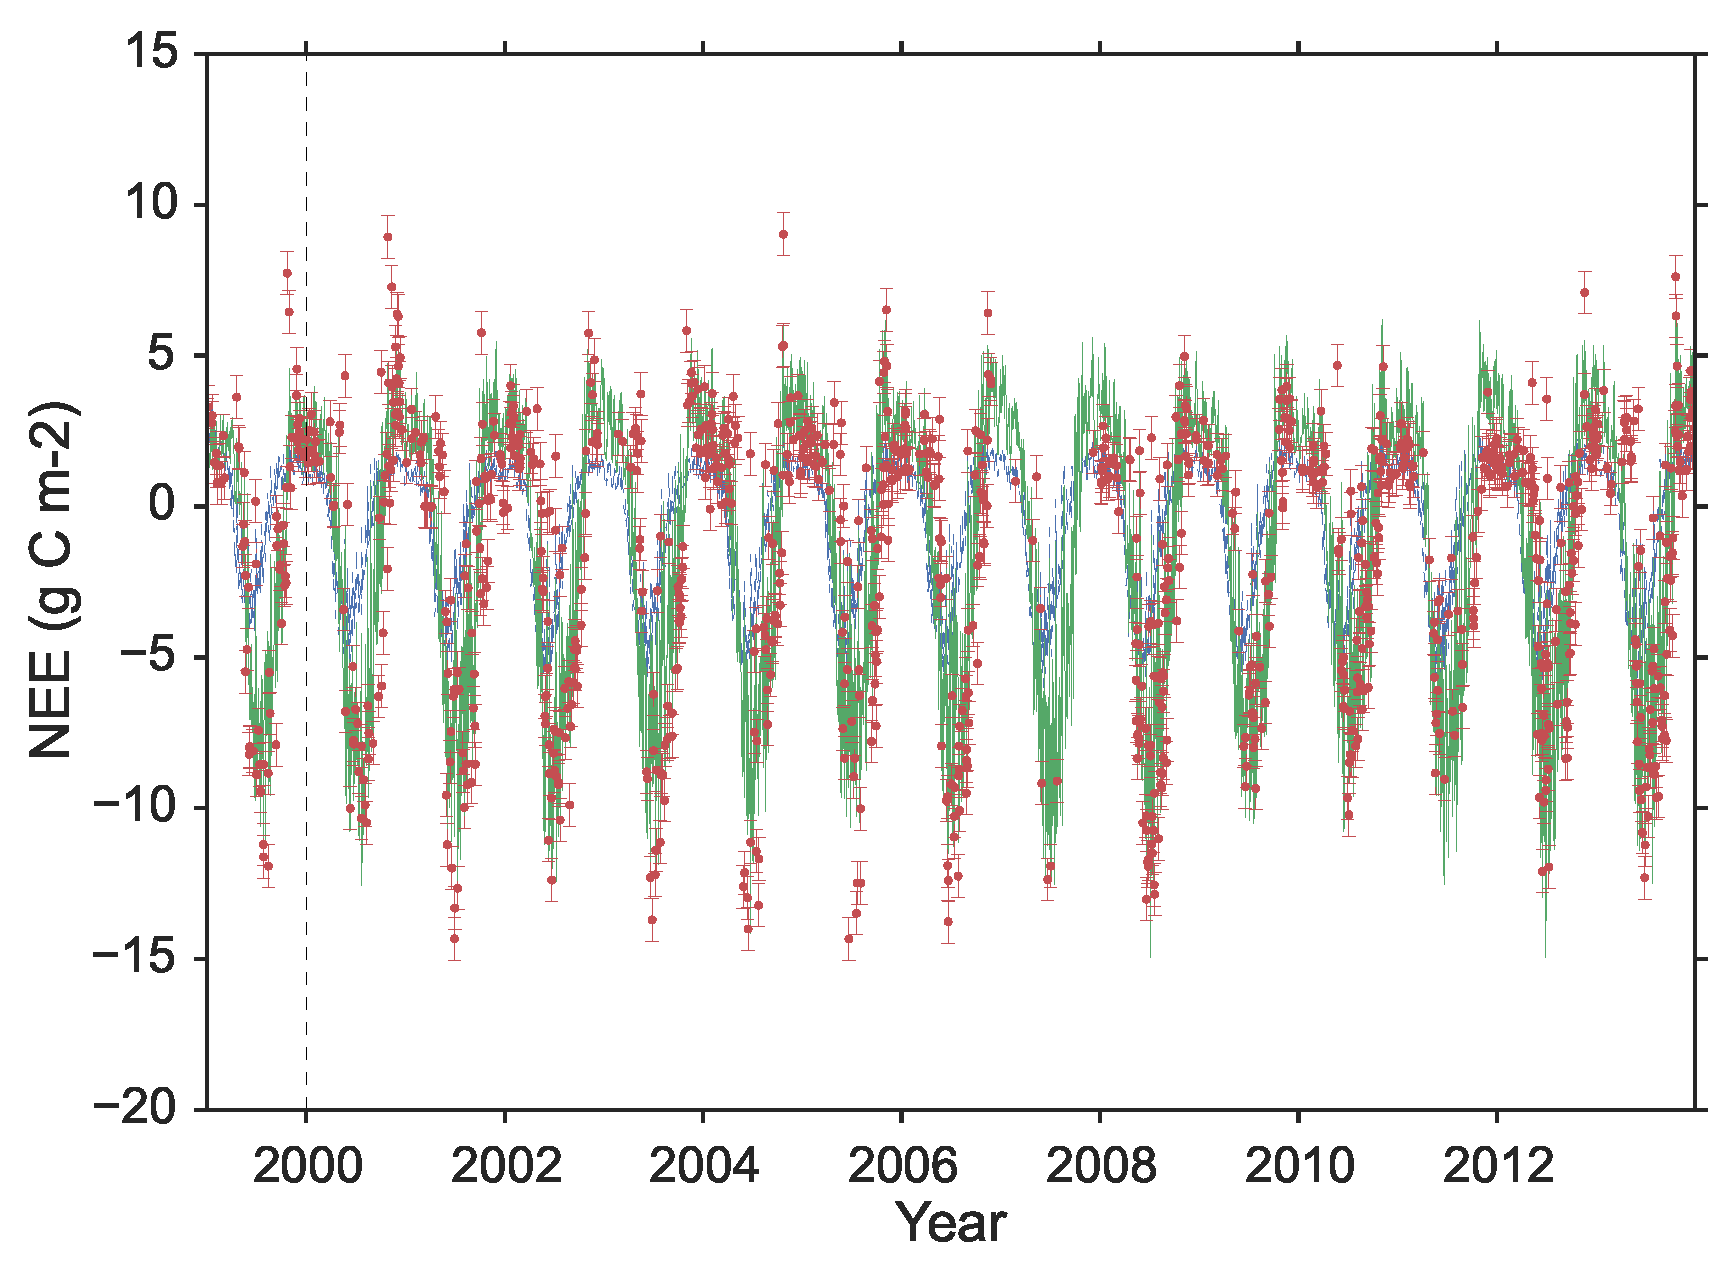
\includegraphics[width=\textwidth]{B4dvar.eps}
        \caption{Experiment B}
        \label{fig:tiger}
    \end{subfigure}
    \begin{subfigure}[b]{0.48\textwidth}
        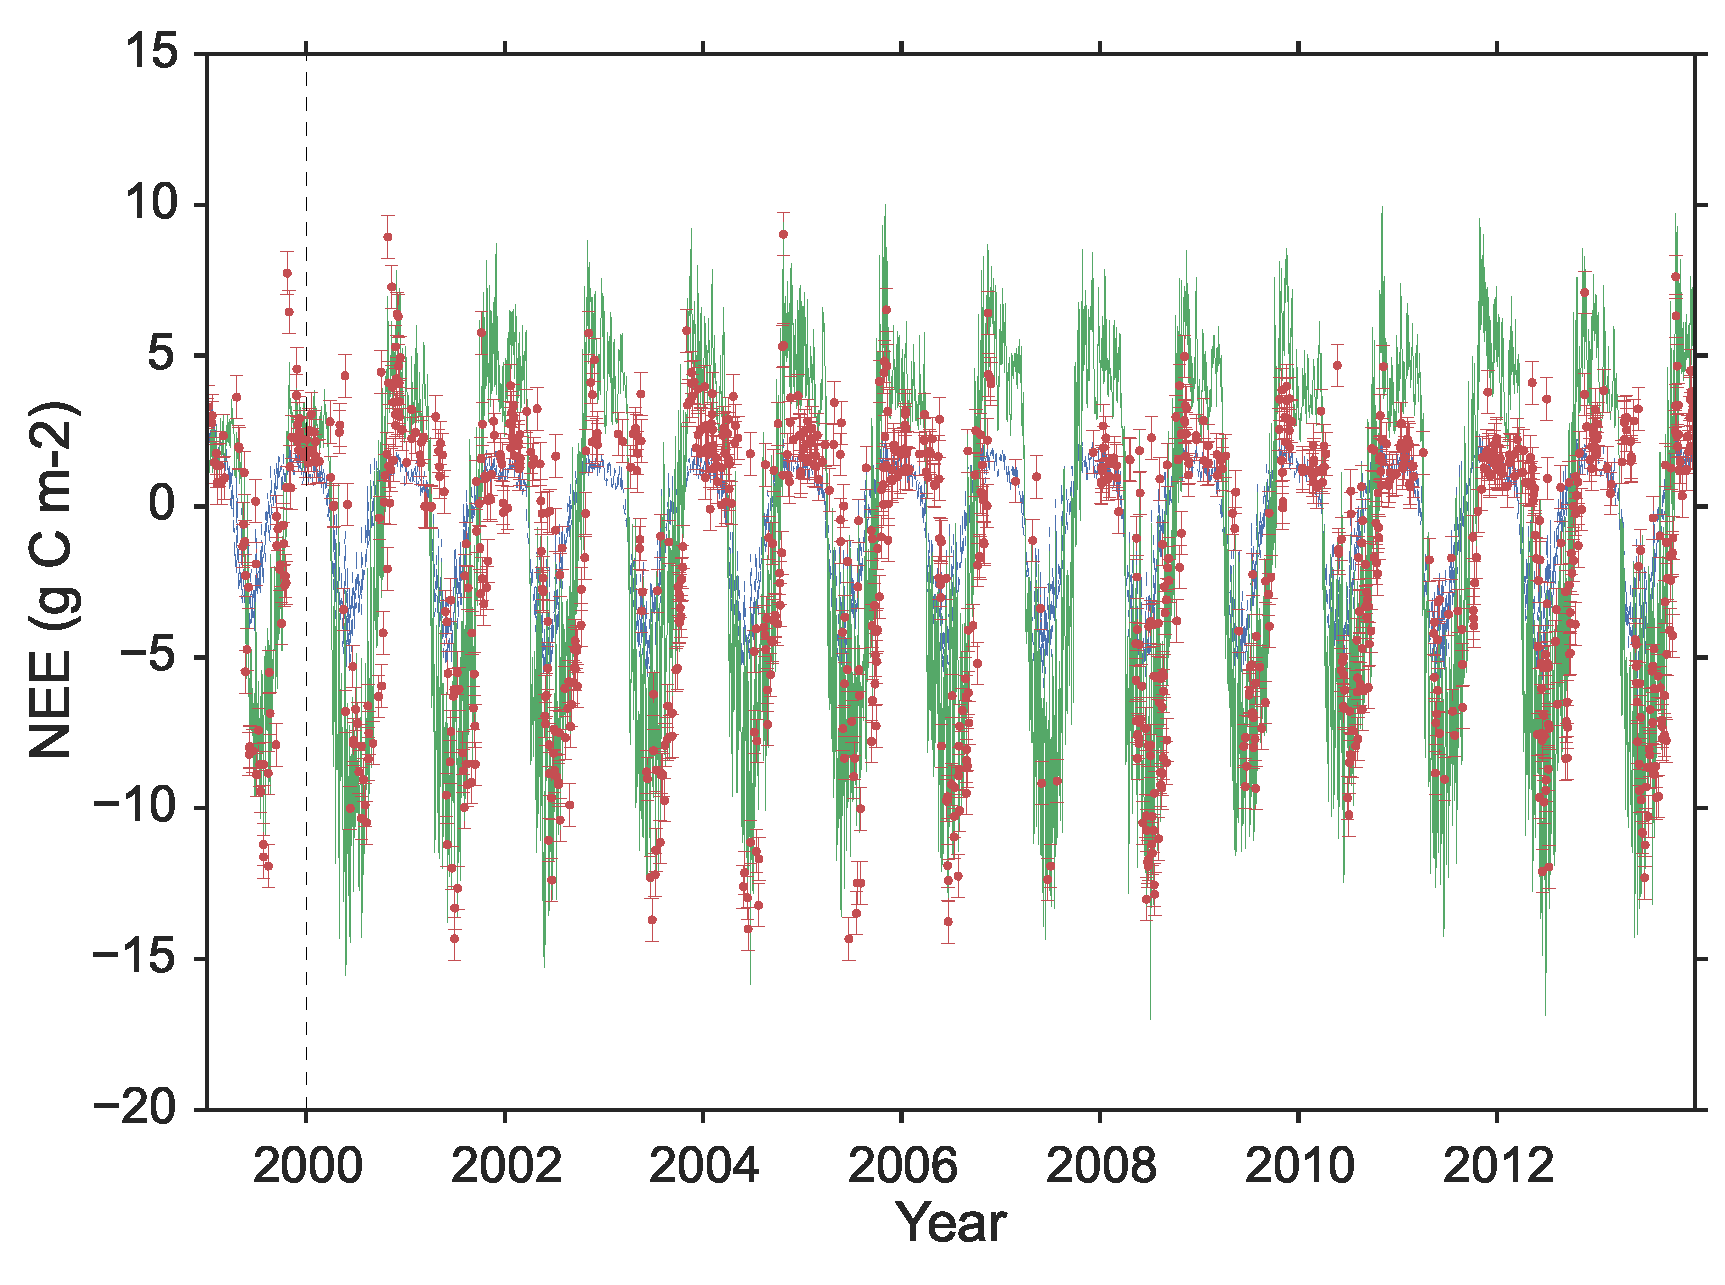
\includegraphics[width=\textwidth]{C4dvar.eps}
        \caption{Experiment C}
        \label{fig:mouse}
    \end{subfigure}
    \begin{subfigure}[b]{0.48\textwidth}
        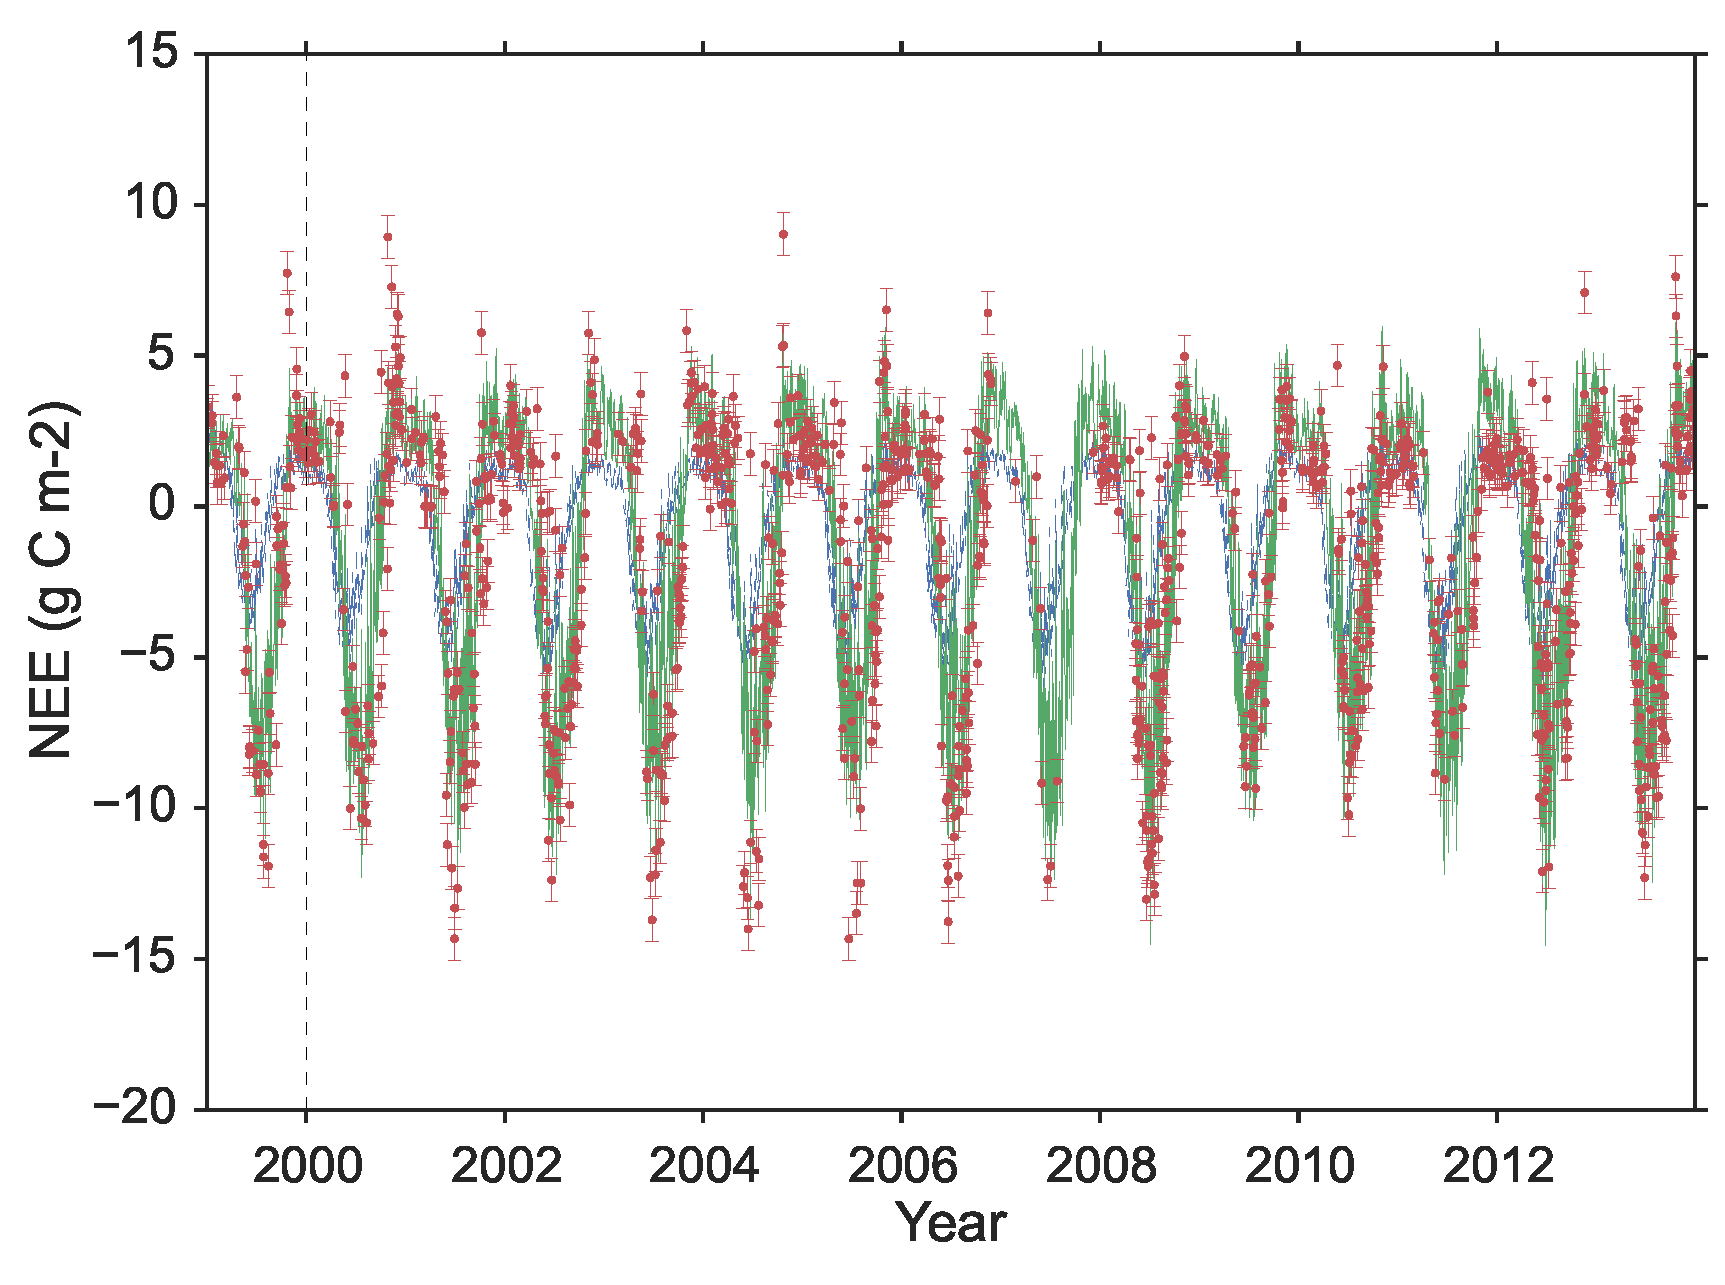
\includegraphics[width=\textwidth]{D4dvar.eps}
        \caption{Experiment D}
        \label{fig:mouse}
    \end{subfigure}
    \caption{One year assimilation and fourteen year forecast of Alice Holt NEE with DALEC2, blue dotted line: background model trajectory, green line: analysis and forecast after assimilation, red dots: observations from Alice Holt flux site with error bars.}\label{fig:animals}
\end{sidewaysfigure}

\begin{figure}
    \centering
    \begin{subfigure}[b]{0.49\textwidth}
        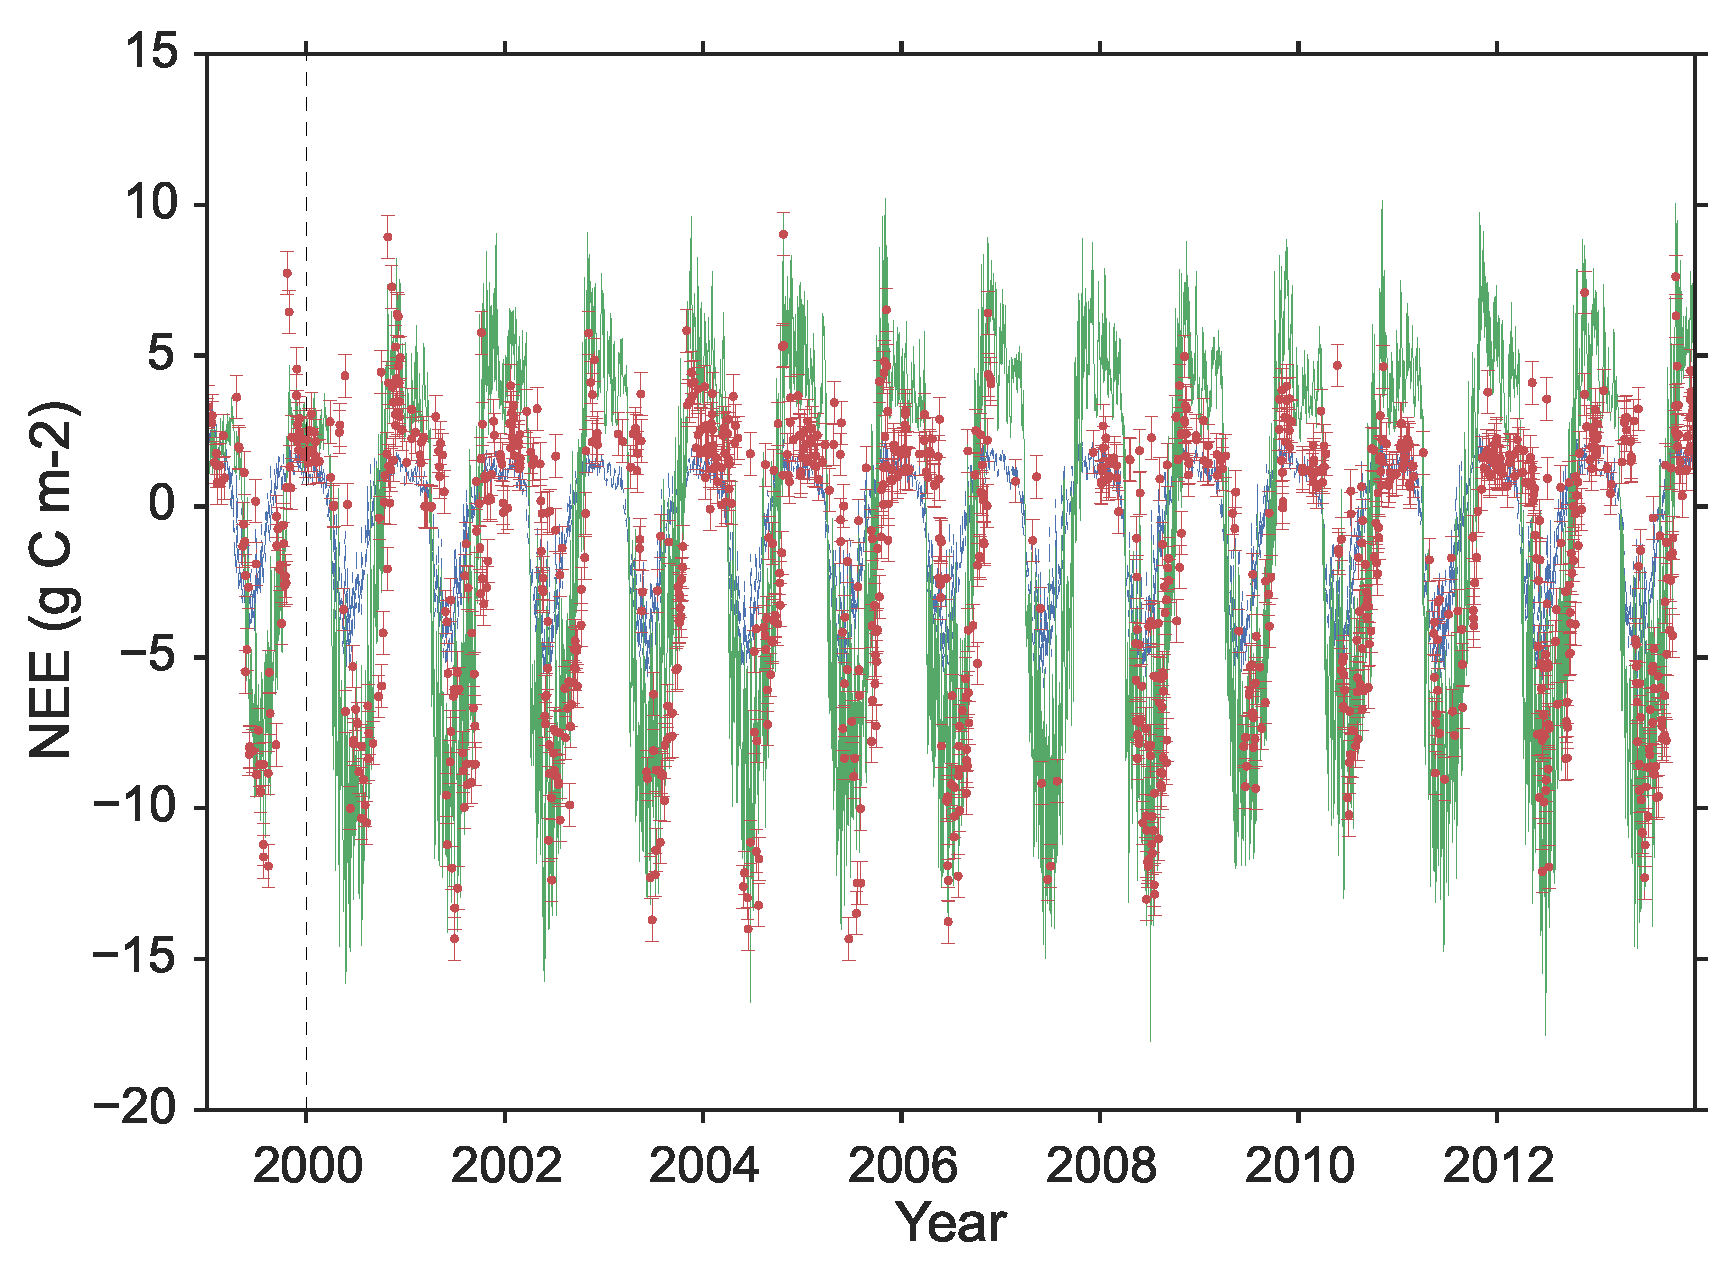
\includegraphics[width=\textwidth]{A4dvar.eps}
        \caption{Experiment A}
        \label{fig:gull}
    \end{subfigure}
    \begin{subfigure}[b]{0.49\textwidth}
        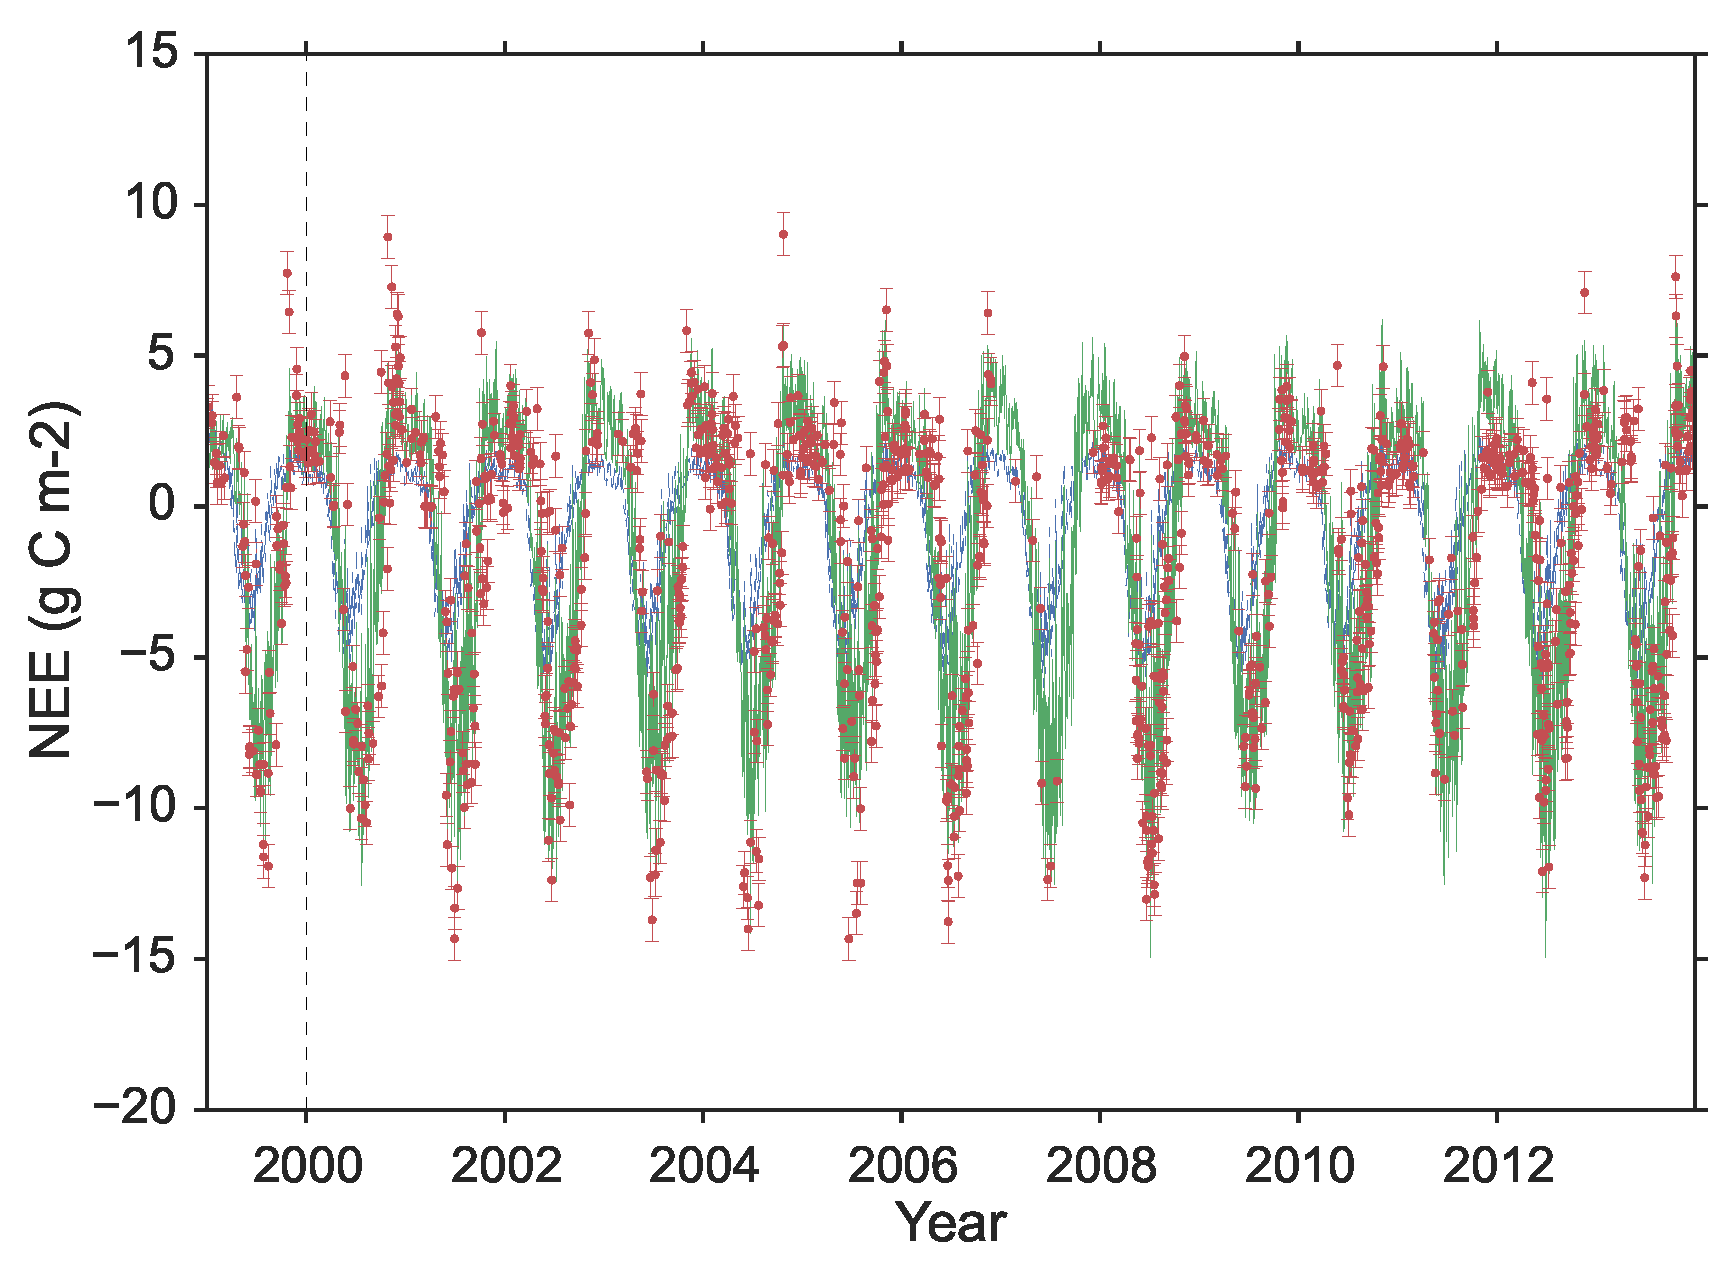
\includegraphics[width=\textwidth]{B4dvar.eps}
        \caption{Experiment B}
        \label{fig:tiger}
    \end{subfigure}
    \begin{subfigure}[b]{0.49\textwidth}
        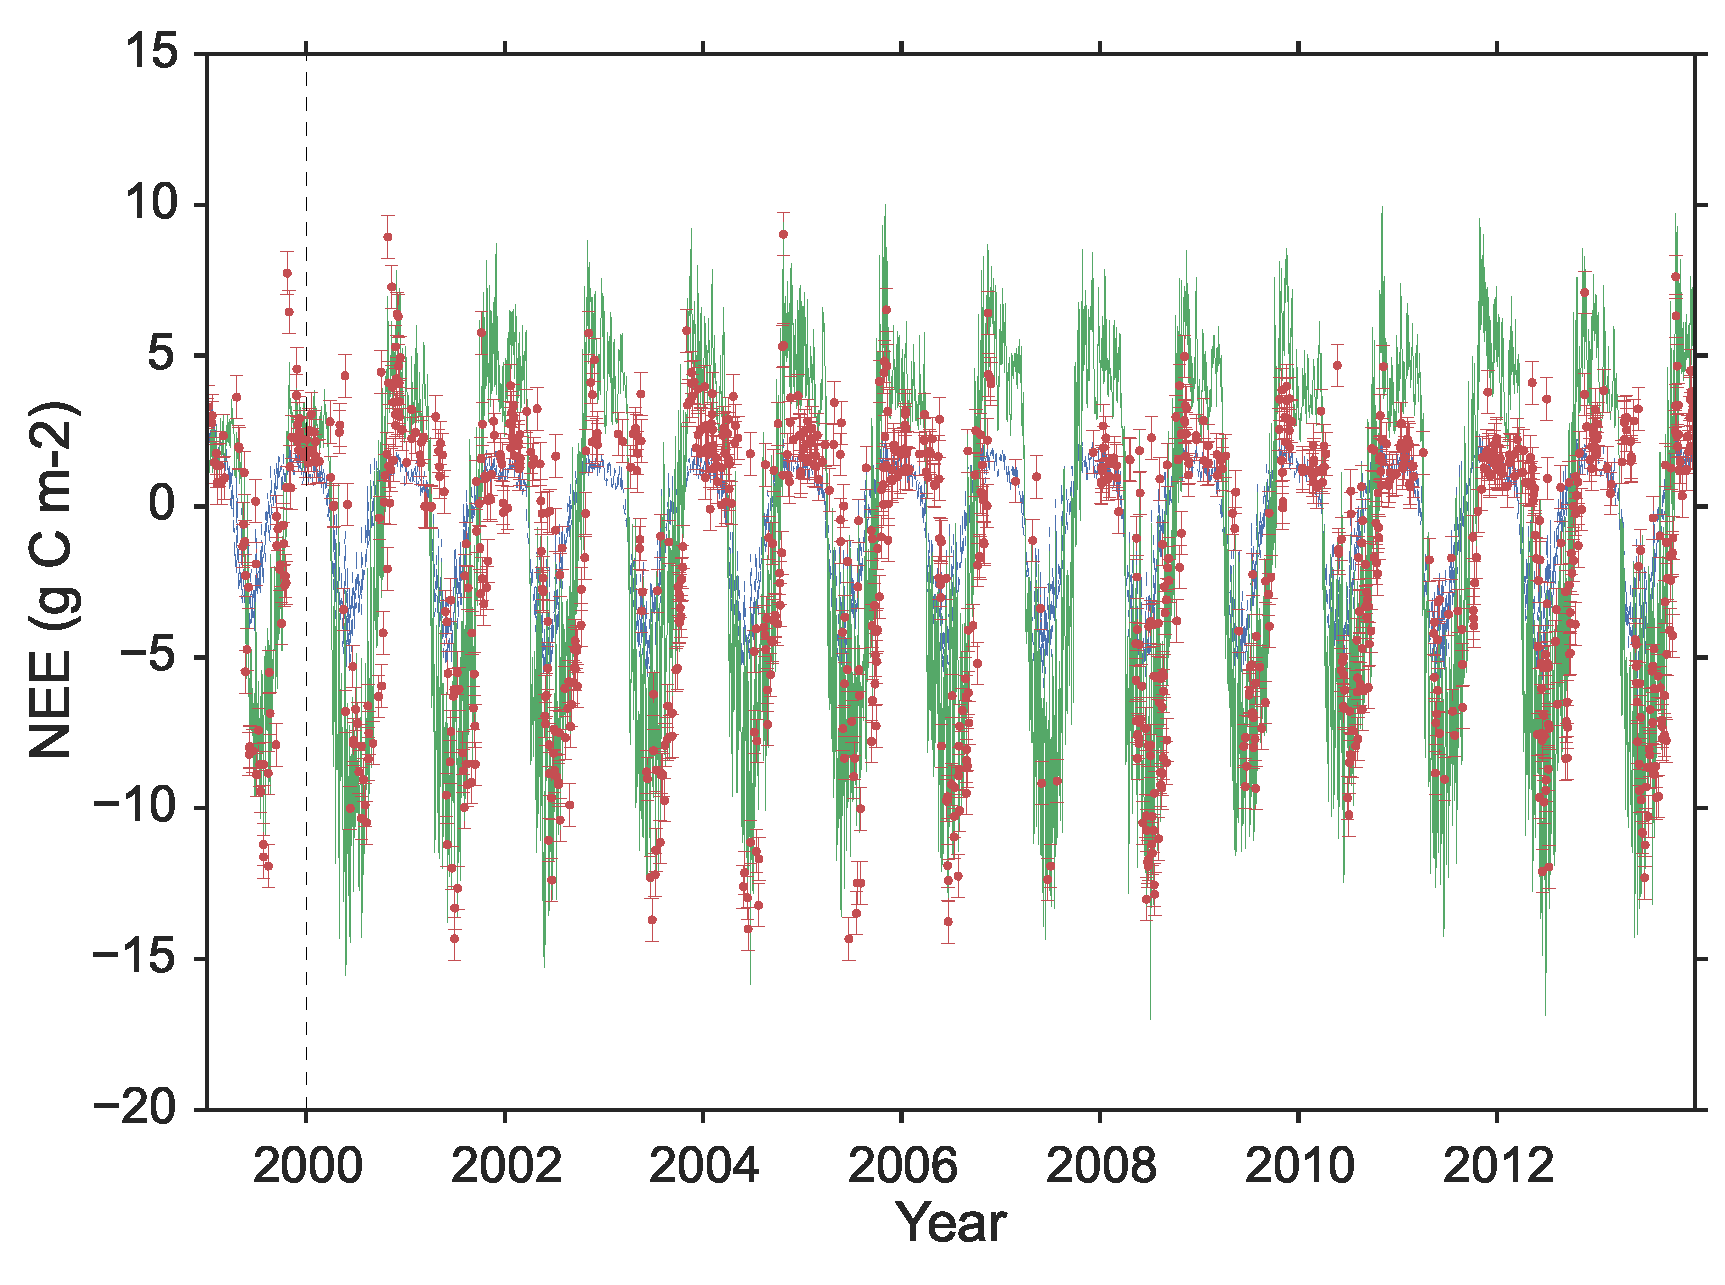
\includegraphics[width=\textwidth]{C4dvar.eps}
        \caption{Experiment C}
        \label{fig:mouse}
    \end{subfigure}
    \begin{subfigure}[b]{0.49\textwidth}
        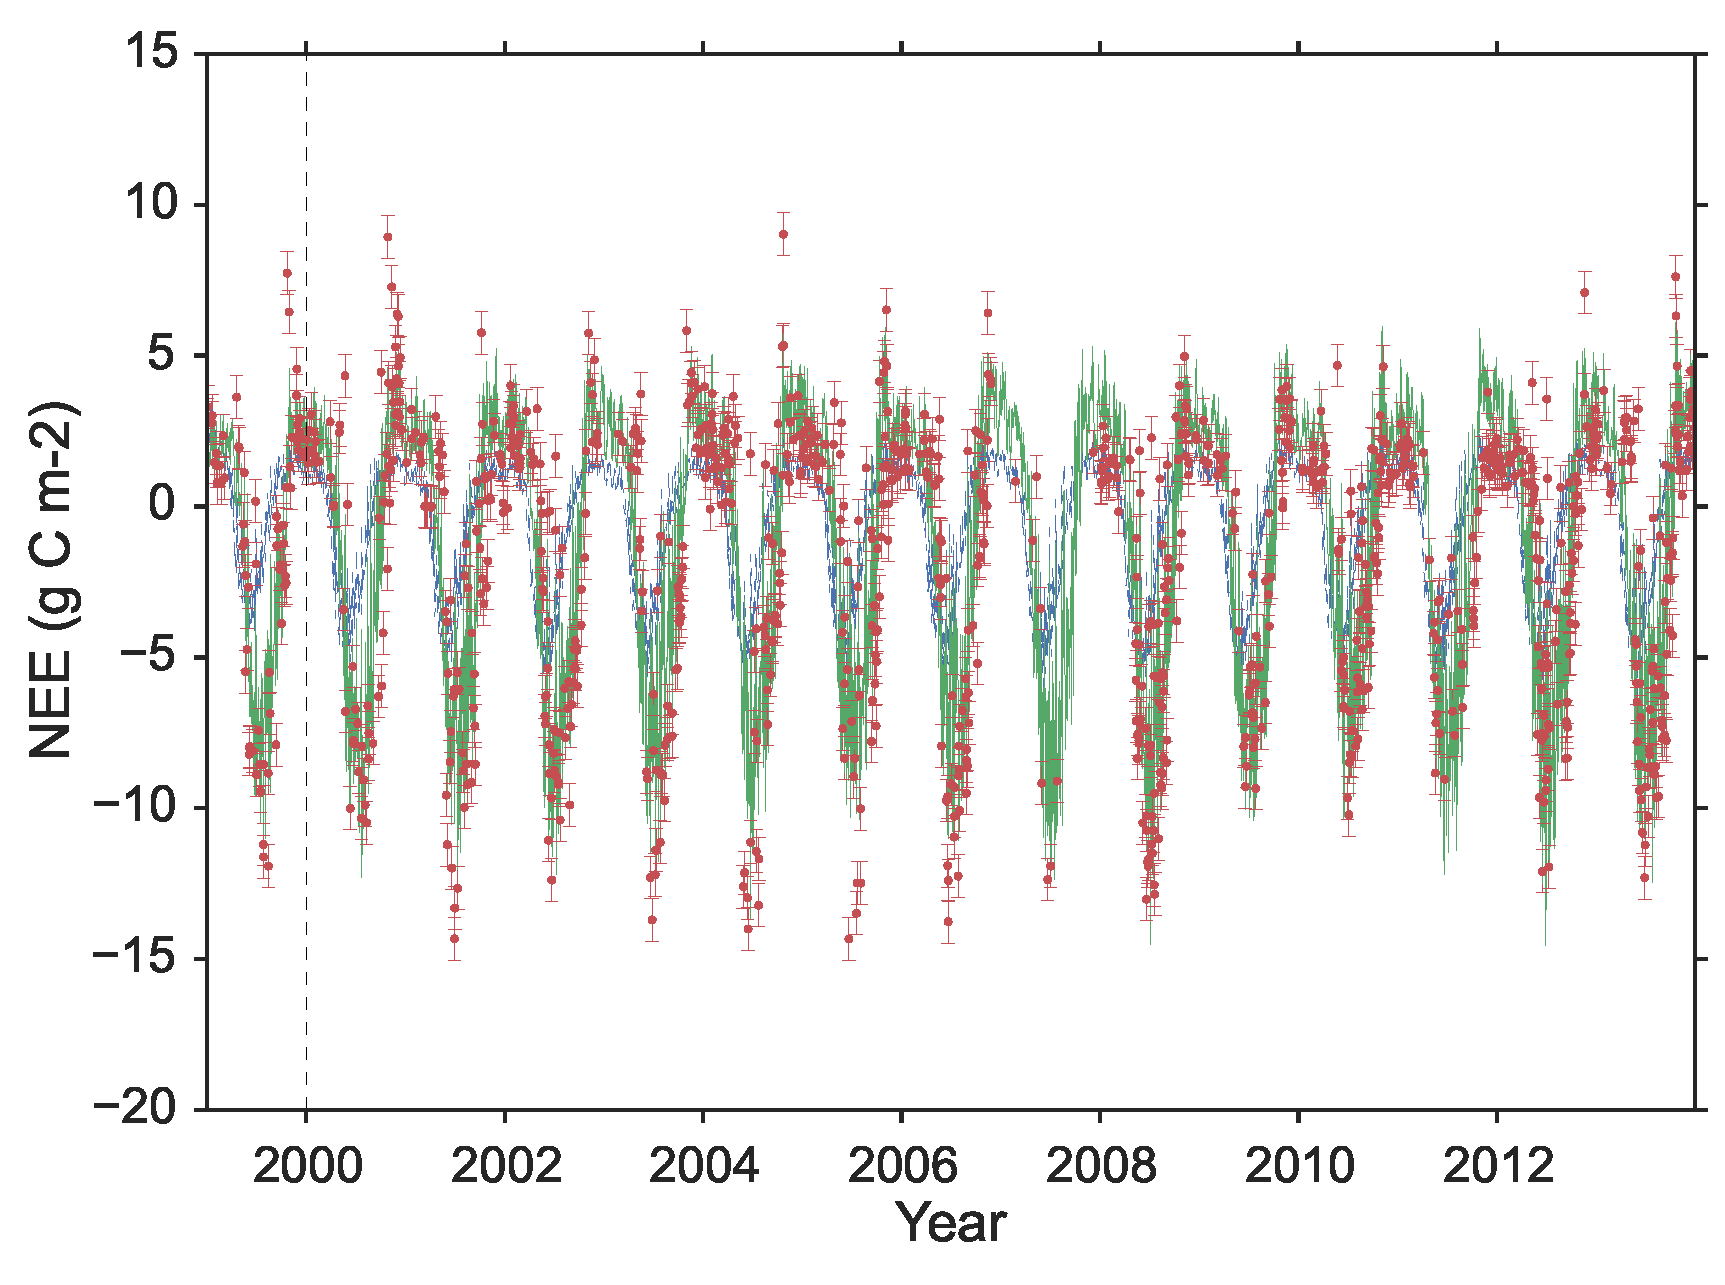
\includegraphics[width=\textwidth]{D4dvar.eps}
        \caption{Experiment D}
        \label{fig:mouse}
    \end{subfigure}
    \caption{One year assimilation and fourteen year forecast of Alice Holt NEE with DALEC2, blue dotted line: background model trajectory, green line: analysis and forecast after assimilation, red dots: observations from Alice Holt flux site with error bars.}\label{fig:animals}
\end{figure}

\begin{figure}
    \centering
    \begin{subfigure}[b]{0.49\textwidth}
        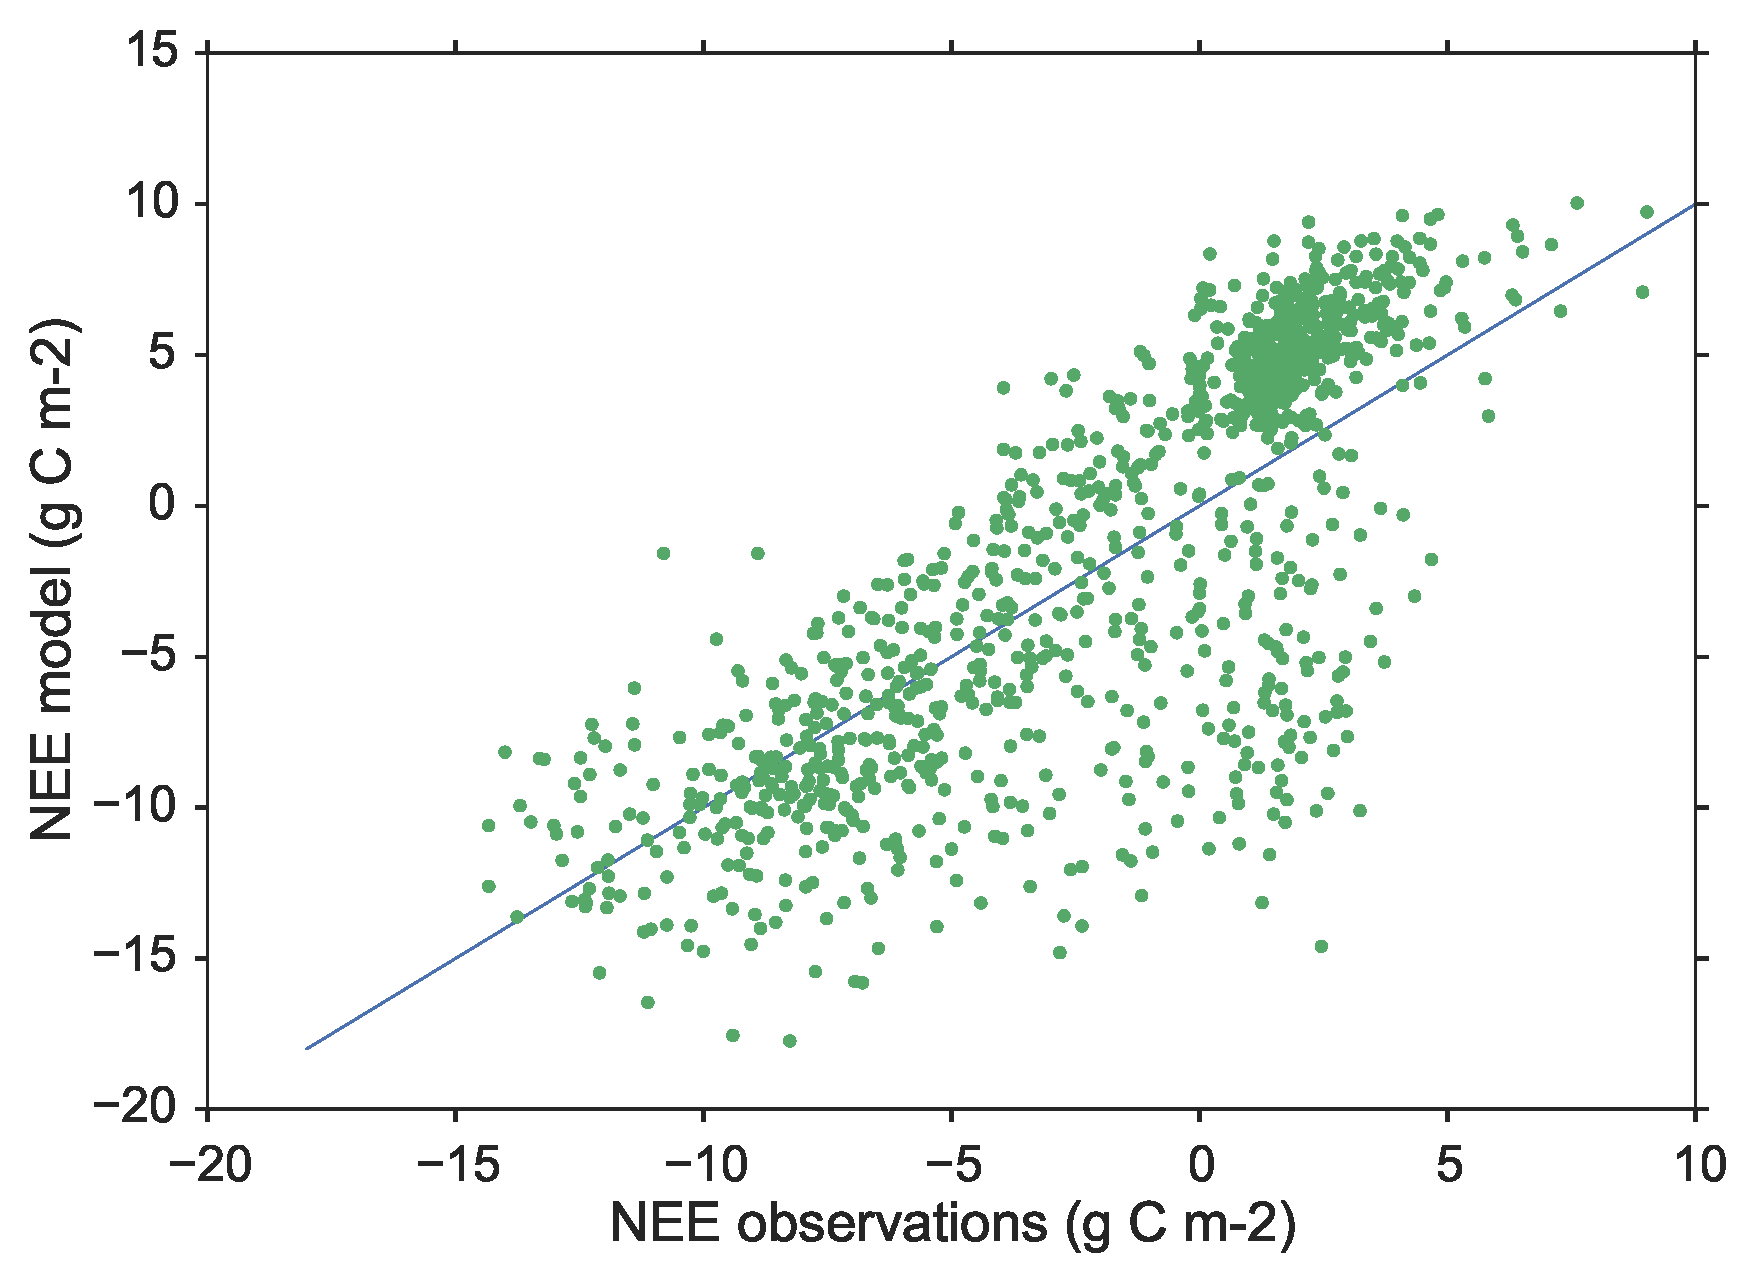
\includegraphics[width=\textwidth]{Afscat.eps}
        \caption{Experiment A}
        \label{fig:gull}
    \end{subfigure}
    \begin{subfigure}[b]{0.49\textwidth}
        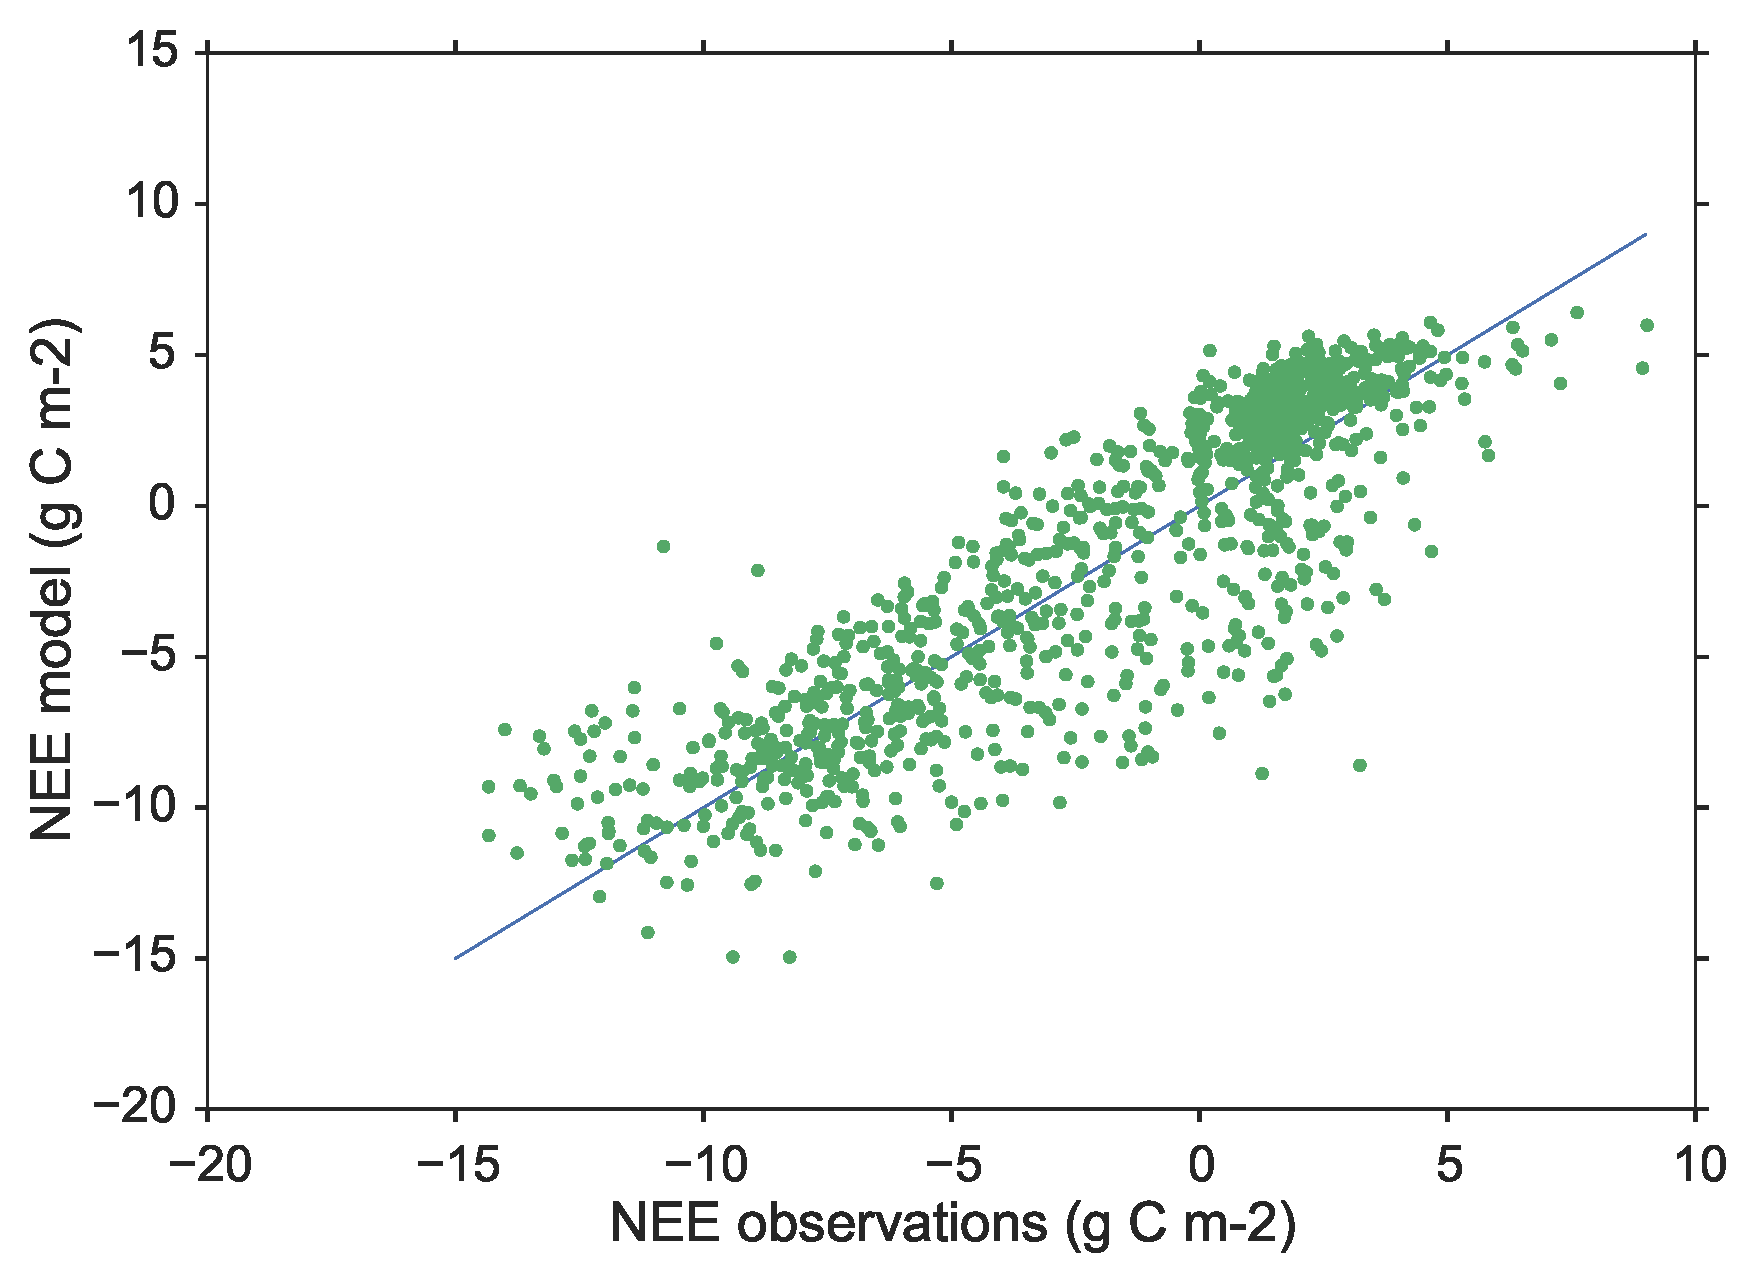
\includegraphics[width=\textwidth]{Bfscat.eps}
        \caption{Experiment B}
        \label{fig:tiger}
    \end{subfigure}
    \begin{subfigure}[b]{0.49\textwidth}
        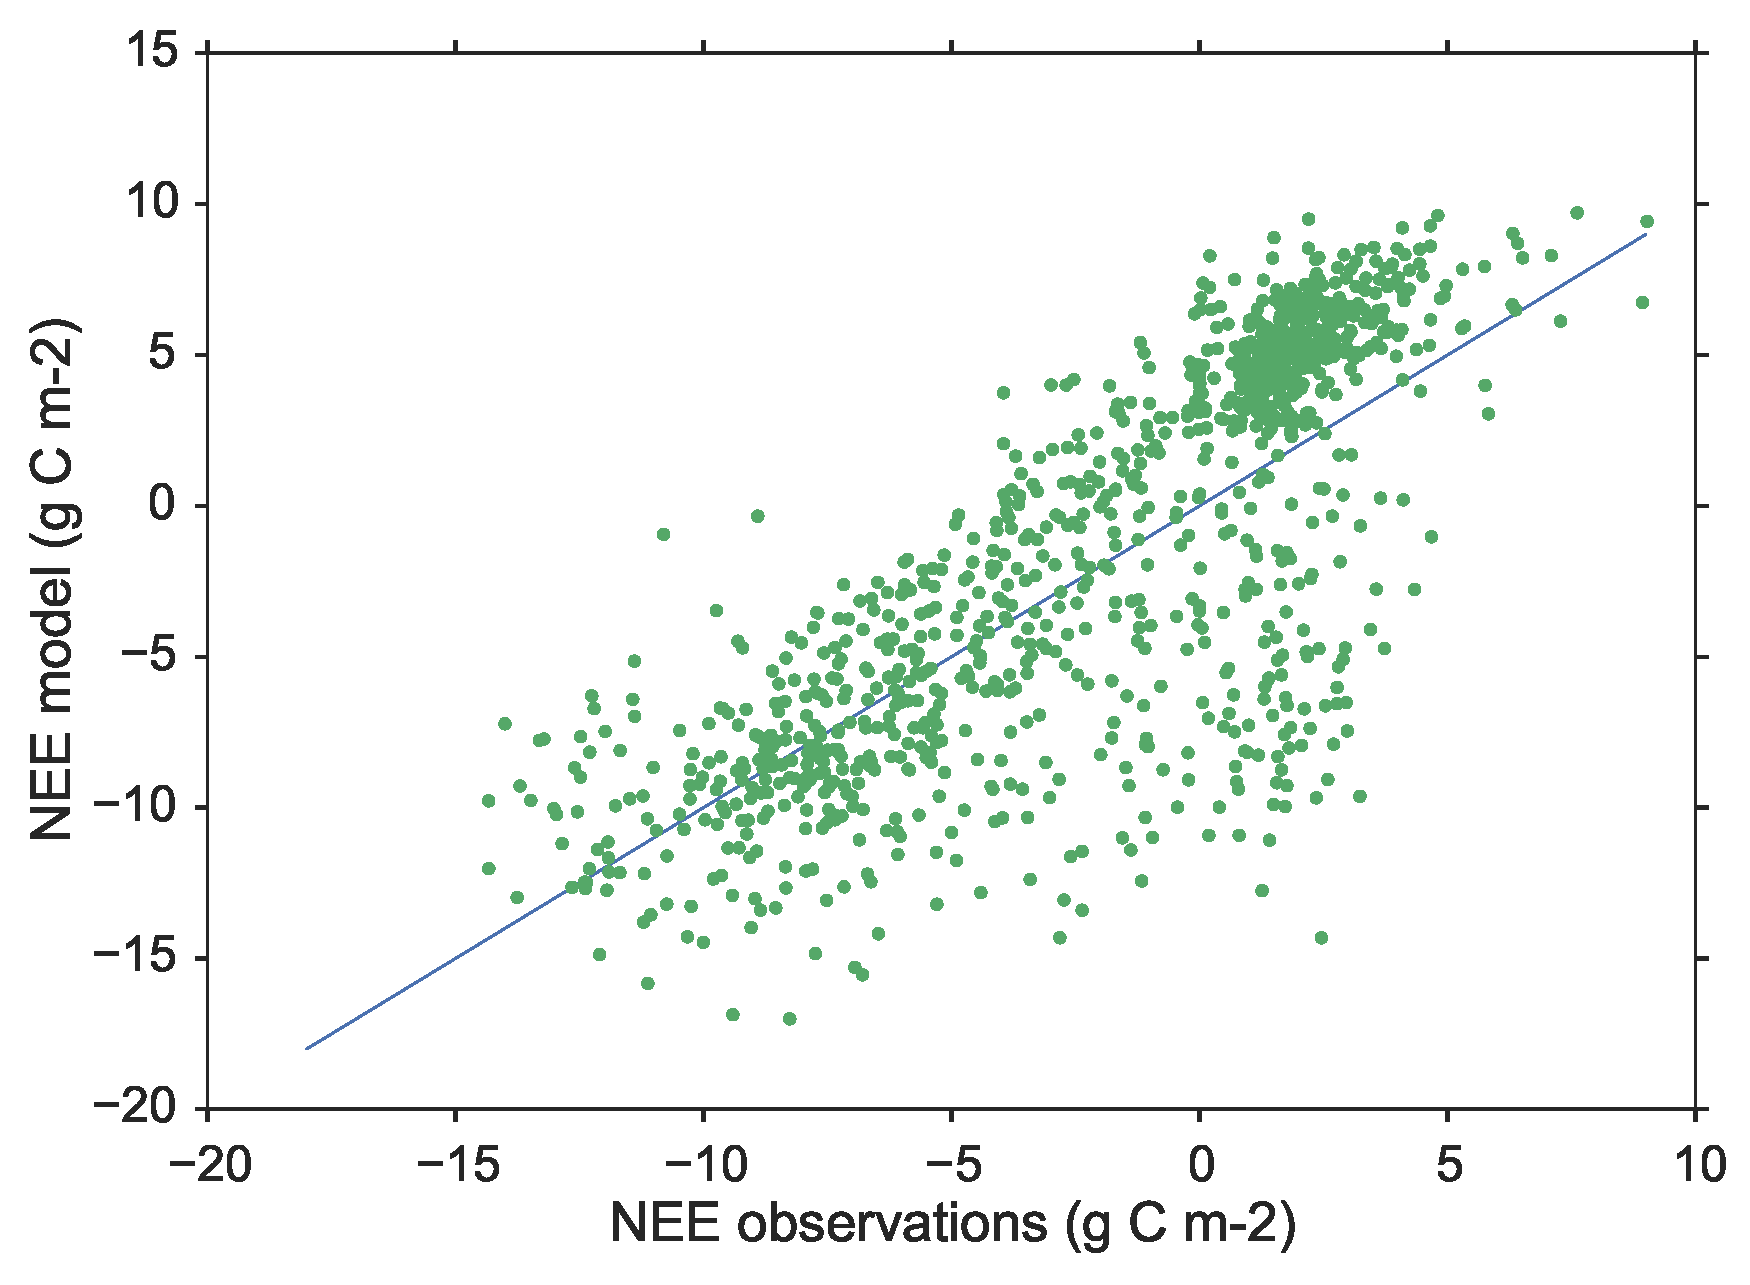
\includegraphics[width=\textwidth]{Cfscat.eps}
        \caption{Experiment C}
        \label{fig:mouse}
    \end{subfigure}
    \begin{subfigure}[b]{0.49\textwidth}
        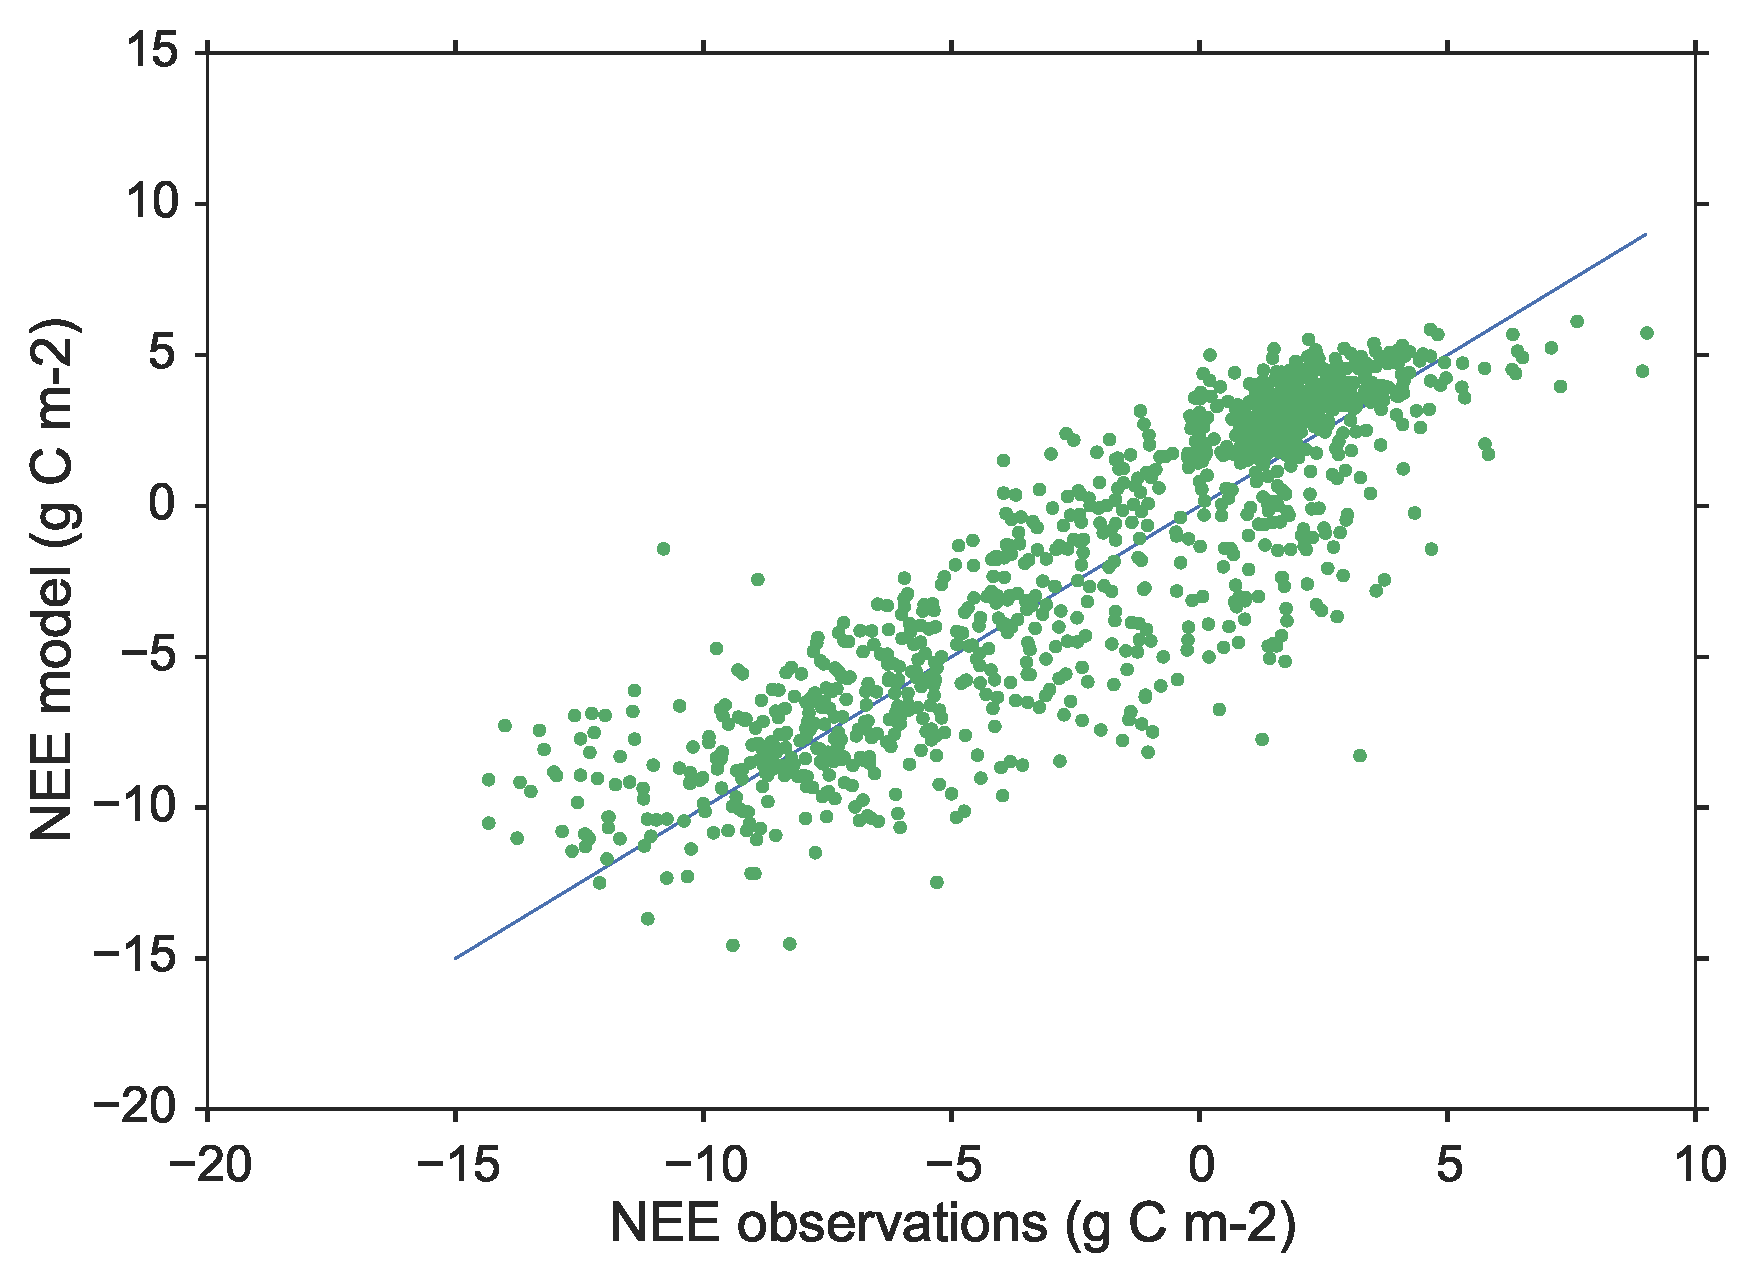
\includegraphics[width=\textwidth]{Dfscat.eps}
        \caption{Experiment D}
        \label{fig:mouse}
    \end{subfigure}
    \caption{Forecast scatter plot of modelled NEE vs. observations for 2000-2014 (green dots). Blue line represents the 1-1 line.}\label{fig:animals}
\end{figure}

\bibliography{../PhD}{}
%\bibliographystyle{plain}

\section*{Appendix}

{\color{red} Write appendix!}

\end{document}